\documentclass[12pt,letterpaper]{article}     	
% Paquetes de generalidades
%%%%%%%%%%%%%%%%%%%%%%%%%%%%%%%

%% Codificación de fuentes correcta
\usepackage[T1]{fontenc} 
% Para escribir tildes y eñes
\usepackage[utf8]{inputenc} 
 % Traduce títulos automáticos al español
\usepackage[spanish]{babel}
% 
\usepackage{parskip}

% Para que la bibligrafía esté en español
\usepackage{babelbib}


% Tamaño del área de escritura de la página	
\usepackage{geometry}                         	\geometry{left=2.5cm,right=2.5cm,top=2.5cm,bottom=2.5cm} 
% Paquetes para matemática
%%%%%%%%%%%%%%%%%%%%%%%%%%%%%%%
% Los paquetes ams son desarrollados por la American Mathematical Society y mejoran la escritura de fórmulas y símbolos matemáticos.
\usepackage{amsmath}       
\usepackage{amsfonts}     	
\usepackage{amssymb}


% Paquetes para manejo de gráficas y figuras
\usepackage{graphicx}   
\usepackage{subcaption}

% Para crear gráficos vectoriales con un lenguaje descriptivo/geométrico
\usepackage{tikz}

% Para crear circuitos vectoriales basados en TikZ
\usepackage[american]{circuitikz}

% Para la presentación correcta de magnitudes y unidades
\usepackage{siunitx}	

% Para hipervínculos y marcadores
\usepackage[colorlinks=true,urlcolor=blue,linkcolor=black,citecolor=green]{hyperref}
	\urlstyle{same}

% Para ubicar las tablas y figuras justo después del texto
\usepackage{float}	

% Para hacer tablas más estilizadas
\usepackage{booktabs}


% Para hacer tablas
\usepackage{tabularx}


% Para hacer secciones con múltiples columnas
\usepackage{multicol}

% Para insertar código fuente estilizado
\usepackage{listings}
	\lstset{basicstyle=\ttfamily,breaklines=true}
    \lstset{numbers=left, numberstyle=\tiny, stepnumber=1, numbersep=6pt}

% Para utilizar el número de páginas
\usepackage{lastpage}

% Para manejar los encabezados y pies de página
\usepackage{fancyhdr}
	% Contenido de los encabezados y pies de pagina
	\pagestyle{fancy}

% Misceláneos
%%%%%%%%%%%%%%%%%%%%%%%%%%%%%%%
% Cita en Formato IEEE
\bibliographystyle{IEEEtran}
% Permite insertar url
\usepackage{url}
% Para insertar símbolos extraños
\usepackage{marvosym}

%%%%%%%%%%%%%%%%%%%%%%%%%%%%%%%%%%%%%%%%%%%%%%%%

% Encabezados
\lhead{Análisis y Diseño del Sistema de Puesta a Tierra}
\chead{}
\rhead{Grupo 4}
 % Pie de pagina
\lfoot{Sistemas de transmisión}
\cfoot{\thepage\ de \pageref{LastPage}}
\rfoot{Universidad Nacional de Colombia}

% Lineas 
\renewcommand{\headrulewidth}{0.4pt}
\renewcommand{\footrulewidth}{0.4pt}

% Comandos especiales
\newcommand{\EIE}{\textsc{Escuela \Lightning~ Ingeniería Eléctrica}}

%%%%%%%%%%%%%%%%%%%%%%%%%%%%%%%%%%%%
\begin{document}
% Portada
\begin{titlepage}
    \centering
    {\scshape\LARGE Universidad Nacional de Colombia - Sede Manizales \par}
    \vspace{0.5cm}
    {\huge\bfseries Análisis del Backflashover y Diseño del Sistema de Puesta a Tierra para una Línea de Subtransmisión de 33 kV Mediante ATPDraw e IEEE Flash\par}
    \vspace{0.5cm}
    {\Large Presentado por: \\
    Maribel Gomez Manchola – Código: 1122732770 \\
    Javier Leonardo Guzmán Olaya – Código: 1108998026 \\
    Juan Jose Marin Mejia – Código: 1055358313 \\
    Juan Esteban Montero Giraldo – Código: 1089379527 \\
    Juan Fernando Montoya Ortiz – Código: 1056121321
   \par}
    \vspace{1cm}
    {\Large \textbf{Profesor:}}\\
    {\Large  Carlos Alberto Quiroz Guarin}\\[2cm]
	{\Large \textbf{Asignatura:}}\\
	{\Large Sistemas de Transmisión}\\[0.5cm]
    \vspace{1cm}
    {\Large Departamento de Ingeniería Eléctrica, Electrónica y Computación\par}
    \vspace{1cm}
    {\Large 16 de Junio de 2026 \par}
\end{titlepage}

\renewcommand{\abstractname}{Resumen} % Cambiamos el nombre del abstract temporalmente

% Portada


% Índice
\tableofcontents

\newpage

\section{Resumen Ejecutivo}

El presente trabajo aborda el análisis del desempeño de una línea de subtransmisión de \SI{33}{\kilo\volt} frente a descargas atmosféricas y el diseño de un sistema de puesta a tierra orientado a reducir la probabilidad de ocurrencia del fenómeno de \textit{Backflashover} (BFO). El estudio se desarrolló sobre la estructura A173 (TORMENTA TIPO R1), considerada como nodo de estudio, e incorporó además las estructuras adyacentes A172 y A174 (ORRECILLA METÁLICA Y TORMENTA TIPO R1) para representar adecuadamente el comportamiento transitorio de la línea.

Para la evaluación del desempeño se emplearon las herramientas ATPDraw e IEEE Flash 2.04, permitiendo analizar la respuesta de la estructura ante impactos directos de rayo y estimar los índices de falla asociados a fenómenos de aislamiento. A partir de los resultados obtenidos se desarrolló un proceso de optimización del sistema de puesta a tierra basado en la utilización de contrapesos horizontales y electrodos verticales.

Como resultado del diseño se identificó una configuración compuesta por dos contrapesos horizontales de \SI{20}{\meter} y un electrodo vertical de \SI{2.4}{\meter}, los cuales proporcionaron una mejora significativa en el comportamiento transitorio de la estructura, manteniendo un equilibrio adecuado entre desempeño eléctrico y viabilidad de implementación.

Los resultados obtenidos evidencian la importancia del diseño del sistema de puesta a tierra como mecanismo de mitigación frente a descargas atmosféricas y demuestran la utilidad de las herramientas de simulación para la evaluación y optimización de redes de subtransmisión.

\section{Introducción}

Las descargas atmosféricas constituyen una de las principales causas de perturbaciones y fallas en los sistemas eléctricos de potencia, particularmente en líneas aéreas de transmisión y subtransmisión. Debido a la elevada magnitud de las corrientes involucradas y a la rápida variación temporal de los fenómenos asociados, los impactos de rayo pueden generar sobretensiones transitorias capaces de comprometer la integridad de los sistemas de aislamiento y afectar la continuidad del servicio eléctrico.

Cuando una descarga atmosférica impacta una estructura o un cable de guarda, la corriente del rayo se propaga a través de la torre y del sistema de puesta a tierra, produciendo elevaciones temporales de potencial que pueden alcanzar valores considerables. Si la diferencia de potencial desarrollada entre la estructura y los conductores de fase supera la capacidad dieléctrica del aislamiento, puede presentarse el fenómeno conocido como \textit{Backflashover} (BFO), el cual constituye uno de los mecanismos más frecuentes de falla asociados a eventos atmosféricos en líneas aéreas.

El desempeño de una estructura frente a este fenómeno depende de diversos factores, entre los que se destacan las características geométricas de la línea, el nivel de aislamiento, la magnitud de la descarga atmosférica y las condiciones del sistema de puesta a tierra. Por esta razón, el diseño adecuado de los elementos destinados a la disipación de corriente hacia el terreno representa una de las estrategias más efectivas para mitigar los efectos de las sobretensiones transitorias y mejorar la confiabilidad de la red.

El análisis de estos fenómenos requiere herramientas especializadas capaces de representar tanto la propagación de ondas electromagnéticas como el comportamiento estadístico de las descargas atmosféricas. En este contexto, ATPDraw permite modelar detalladamente los elementos que conforman la línea y evaluar su respuesta frente a eventos transitorios, mientras que IEEE Flash proporciona metodologías para estimar índices de desempeño relacionados con fallas por descargas atmosféricas.

La combinación de estas herramientas constituye una base sólida para el estudio de fenómenos de alta frecuencia y para el desarrollo de soluciones orientadas al mejoramiento del comportamiento de las líneas frente a eventos atmosféricos, contribuyendo al incremento de la confiabilidad y disponibilidad de los sistemas eléctricos de potencia.


\section{Objetivos}

\subsection{Objetivo General}
Analizar el desempeño de un tramo de línea de subtransmisión de $\SI{33}{\kV}$ (estructuras A170 a A176) frente a descargas atmosféricas y diseñar un sistema de puesta a tierra óptimo mediante herramientas de simulación transitoria y estadística, con el fin de mitigar las salidas de línea debidas al fenómeno de Backflashover bajo criterios técnicos.

\subsection{Objetivos Específicos}
\begin{itemize}
    \item Determinar analíticamente los parámetros modales de secuencia cero y positiva del tramo de línea asignado para su correcta parametrización en el programa Line Constants (LCC) de ATPDraw.
    \item Evaluar estadísticamente la tasa anual de salidas y fallas por apantallamiento y backflashover del caso base de la línea empleando el software IEEE Flash 2.04.
    \item Desarrollar un modelo electromagnético detallado en el dominio del tiempo en ATPDraw que represente fielmente el nodo de estudio, los apoyos adyacentes, la función de onda de corriente del rayo (Heidler) y el comportamiento no lineal del aislamiento mediante el criterio Volt-Time.
    \item Diseñar de manera iterativa diversas configuraciones de sistemas de puesta a tierra empleando combinaciones de contrapesos horizontales y electrodos verticales.
\end{itemize}

\section{Alcance del Proyecto}

El presente trabajo comprende el análisis del comportamiento de una estructura perteneciente a una línea de subtransmisión de \SI{33}{\kilo\volt} frente a descargas atmosféricas, así como el diseño de un sistema de puesta a tierra orientado a mejorar su desempeño ante el fenómeno de \textit{Backflashover} (BFO). El estudio se centra en la estructura A173, seleccionada como nodo de estudio, debido a su ubicación dentro del tramo asignado para el desarrollo de este proyecto.

Con el fin de representar adecuadamente la propagación y reflexión de las ondas transitorias generadas por una descarga atmosférica, el modelo electromagnético incluyó las estructuras comprendidas entre los apoyos A170 y A176. Las estructuras A172, A173 y A174, correspondientes a la zona de influencia directa del nodo de estudio, fueron representadas mediante modelos detallados de alta frecuencia. Para estas estructuras se incorporó la geometría suministrada mediante la modelación explícita de las crucetas, bayonetas, cadenas de aisladores, impedancias de la torre y sistemas de puesta a tierra asociados. Las estructuras restantes se representaron mediante modelos equivalentes simplificados, permitiendo incluir el efecto de los tramos adyacentes dentro del comportamiento global de la línea.


El trabajo contempla la determinación de los parámetros eléctricos de los diferentes tramos de línea, la modelación de las estructuras seleccionadas, la evaluación del desempeño frente a descargas atmosféricas mediante ATPDraw e IEEE Flash 2.04, y el diseño de alternativas de puesta a tierra basadas en contrapesos horizontales y electrodos verticales.

No forman parte del alcance del presente estudio las modificaciones en la geometría de la línea, los cambios en los niveles de aislamiento, la incorporación de descargadores de sobretensión, la coordinación de aislamiento de subestaciones ni el análisis de otros mecanismos de falla diferentes al \textit{Backflashover}. Asimismo, las características eléctricas del terreno y de los conductores se consideran constantes y corresponden a los datos suministrados para el caso de estudio.


\section{Marco Teórico}

\subsection{Descargas Atmosféricas en Líneas de Subtransmisión}


\subsubsection{Densidad de Descargas a Tierra ($N_g$) y Modelo Estadístico de Poisson}
La evaluación del desempeño de una línea de subtransmisión frente a descargas atmosféricas requiere la caracterización estadística de la actividad eléctrica de la región donde se encuentra emplazada. El parámetro más utilizado para este propósito es la densidad de descargas a tierra, denotada por ($N_g$), la cual representa el número promedio anual de descargas atmosféricas que impactan una superficie de un kilómetro cuadrado y constituye un indicador de la severidad atmosférica de una zona determinada \cite{ieee1410}.

Debido a que la ocurrencia de descargas atmosféricas corresponde a un fenómeno aleatorio y discreto tanto en el tiempo como en el espacio, la frecuencia de impactos sobre una infraestructura eléctrica suele modelarse mediante un proceso de Poisson. Bajo esta aproximación, se asume que los eventos ocurren de forma independiente y con una tasa media constante dentro del intervalo de análisis. La probabilidad de que ocurran exactamente (k) eventos durante dicho intervalo está dada por:

\begin{equation}
P(k)=\frac{e^{-\lambda}\lambda^k}{k!}
\label{eq:poisson}
\end{equation}

donde (k) corresponde al número de descargas atmosféricas consideradas y ($\lambda$) representa el número esperado de eventos. En estudios de desempeño atmosférico de líneas aéreas, este parámetro se relaciona con la densidad de descargas a tierra y el área de exposición equivalente de la estructura mediante:

\begin{equation}
\lambda=N_g,A_e
\label{eq:lambda}
\end{equation}

siendo ($A_e$) el área efectiva de captura de la línea o estructura analizada.

La probabilidad acumulada de que ocurran como máximo (m) eventos se obtiene mediante la suma de las probabilidades individuales:

\begin{equation}
P(k\leq m)=\sum_{k=0}^{m}\frac{e^{-\lambda}\lambda^k}{k!}
\label{eq:poisson_acum}
\end{equation}

\begin{figure}[H]
    \centering
    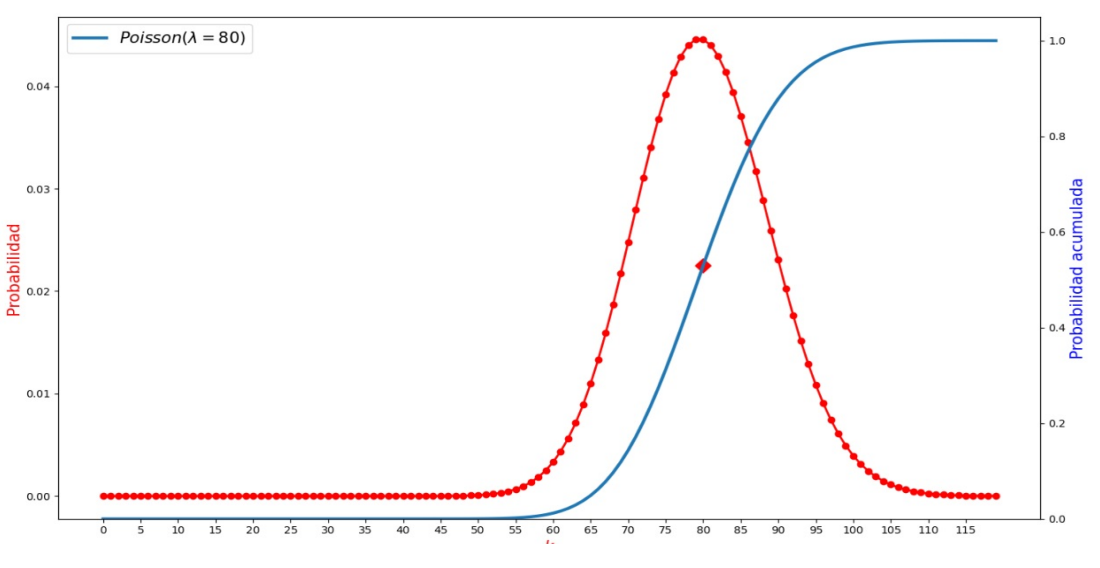
\includegraphics[width=0.75\textwidth]{Figs/Marco teorico/poisson_fig.png}
    \caption{Función de probabilidad y probabilidad acumulada para una distribución de Poisson con parámetro $\lambda$.}
    \label{fig:poisson_distribution}
\end{figure}

La Figura \ref{fig:poisson_distribution} ilustra el comportamiento típico de una distribución de Poisson y su correspondiente probabilidad acumulada. Puede observarse que la mayor concentración de probabilidad se presenta alrededor del valor esperado $\lambda$, mientras que la función acumulada converge progresivamente hacia la unidad a medida que aumenta el número de eventos considerados.

\subsubsection{Mecanismos de Falla: \textit{Flashover} frente a \textit{Backflashover} (BFO)}

Las descargas atmosféricas pueden generar sobretensiones transitorias capaces de superar la capacidad de soportabilidad de las cadenas de aisladores de una línea aérea. Cuando esto ocurre, se produce una ruptura dieléctrica del aislamiento conocida como \textit{Flashover}, estableciéndose un arco eléctrico entre puntos con diferente potencial.

Dependiendo del origen de la sobretensión, pueden distinguirse diferentes mecanismos de falla. El \textit{Flashover} convencional ocurre cuando una descarga impacta directamente un conductor de fase o induce sobre éste una sobretensión suficiente para provocar la ruptura del aislamiento hacia la estructura puesta a tierra \cite{IEEE_1243}.

Por otra parte, el \textit{Backflashover} (BFO) se presenta cuando una descarga impacta una estructura o el cable de guarda, produciendo una elevación transitoria del potencial de la torre. Si la diferencia de potencial entre la estructura y los conductores de fase supera la capacidad dieléctrica del aislamiento, se desarrolla un arco desde la torre hacia el conductor de fase.

La Figura \ref{fig:backflashover} muestra de manera conceptual este mecanismo de falla. Puede observarse cómo la corriente del rayo se conduce a través de la estructura, generando una elevación de potencial que eventualmente produce la ruptura del aislamiento.

\begin{figure}[H]
\centering
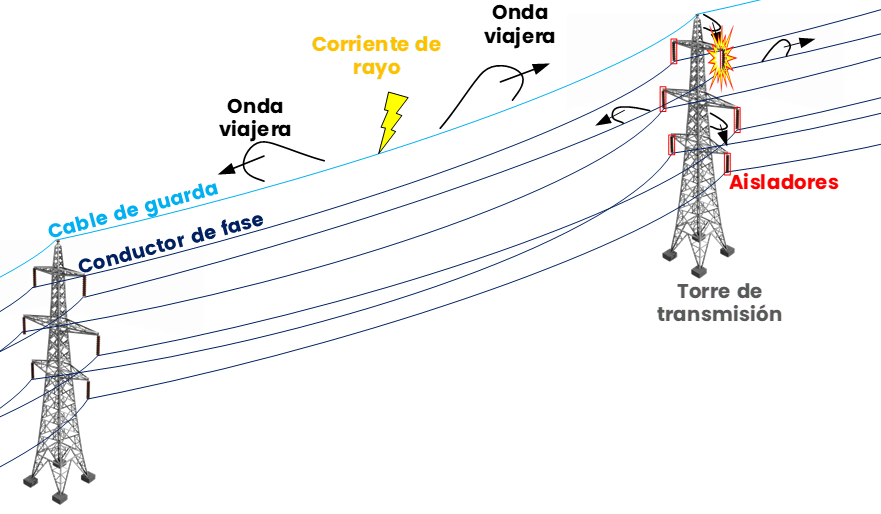
\includegraphics[width=0.65\textwidth]{Figs/Marco teorico/BFO.png}
\caption{Representación conceptual del fenómeno de \textit{Backflashover} ocasionado por el impacto de una descarga atmosférica sobre el cable de guarda de una línea aérea.}
\label{fig:backflashover}
\end{figure}

Dado que el \textit{Backflashover} constituye uno de los mecanismos predominantes de falla en líneas protegidas mediante cables de guarda, su análisis y mitigación resultan fundamentales para el diseño de sistemas de puesta a tierra y para la mejora del desempeño atmosférico de las estructuras de subtransmisión.


\subsection{Propagación de Ondas Transitorias y Mecanismos de Ruptura Dieléctrica}

\subsubsection{Sobretensiones por Impacto Directo y Ondas Viajeras}
Cuando una descarga atmosférica impacta una estructura o el cable de guarda de una línea aérea, la corriente inyectada no se distribuye instantáneamente a lo largo del sistema, sino que se propaga en forma de ondas electromagnéticas transitorias. Estas ondas viajeras transportan energía a través de los conductores y estructuras, produciendo variaciones temporales de tensión y corriente que difieren significativamente de las condiciones de operación en régimen permanente.

En el caso de impactos sobre el cable de guarda, la corriente del rayo se distribuye entre las estructuras adyacentes y los sistemas de puesta a tierra, generando elevaciones transitorias de potencial sobre las torres. Estas sobretensiones pueden alcanzar valores suficientemente elevados para comprometer la capacidad dieléctrica del aislamiento y dar origen a fenómenos de \textit{Backflashover}.


\subsubsection{Modelo de Ruptura No Lineal del Aislamiento (Criterio Volt-Time)}

La respuesta del aislamiento frente a sobretensiones atmosféricas presenta un comportamiento no lineal, ya que la ruptura dieléctrica depende tanto de la magnitud de la tensión aplicada como del tiempo durante el cual ésta actúa sobre el aislamiento. Por esta razón, la soportabilidad no puede describirse mediante un único valor de tensión crítica.

Para representar este fenómeno se emplea el criterio \textit{Volt-Time}, el cual establece una relación entre la tensión aplicada y el tiempo necesario para que ocurra la ruptura del aislamiento. En general, sobretensiones de mayor amplitud producen la descarga disruptiva en intervalos de tiempo más cortos.

La Figura \ref{fig:volttime} muestra una representación conceptual de esta característica. Durante una simulación transitoria, la tensión desarrollada sobre la cadena de aisladores se compara continuamente con la curva de soportabilidad. Cuando la solicitación supera dicho límite, se considera que ocurre un fenómeno de \textit{Flashover} o \textit{Backflashover}.
\begin{figure}[H]
    \centering
    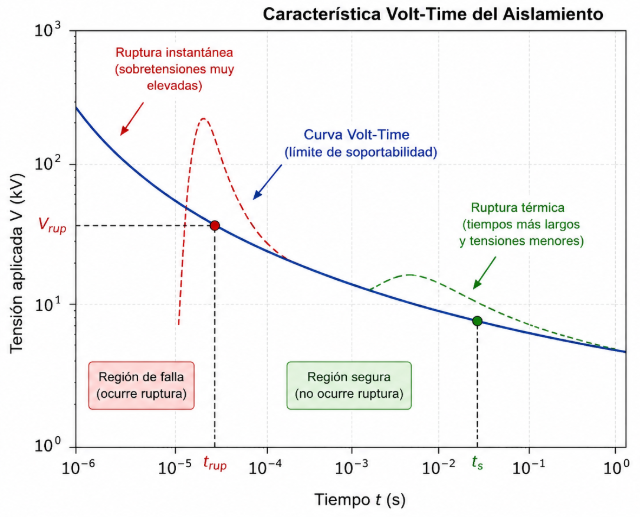
\includegraphics[width=0.55\textwidth]{Figs/Marco teorico/Volt.png}
    \caption{Representación conceptual de la característica \textit{Volt-Time} de una cadena de aisladores. La ruptura ocurre cuando la combinación de tensión aplicada y tiempo de exposición supera la curva de soportabilidad del aislamiento.}
    \label{fig:volttime}
\end{figure}

Este criterio es ampliamente utilizado en estudios de desempeño atmosférico, ya que permite representar de manera realista el comportamiento del aislamiento ante impulsos de rayo y evaluar la probabilidad de falla bajo condiciones transitorias.

\subsection{Modelado de Elementos en Alta Frecuencia}

\subsubsection{Representación de la Corriente del Rayo: Función de Heidler}

Para el modelado transitorio de descargas atmosféricas en \textsc{ATPDraw}, la corriente del rayo se representa mediante la función de Heidler. Este modelo matemático reproduce con precisión el rápido crecimiento del frente de onda impulsivo y su posterior decaimiento mediante la Ecuación \eqref{eq:heidler}:

\begin{equation}
i(t)=\frac{I_0}{\eta} \cdot \frac{\left(\frac{t}{\tau_1}\right)^n}{1+\left(\frac{t}{\tau_1}\right)^n} \cdot e^{-t/\tau_2}
\label{eq:heidler}
\end{equation}

donde $I_0$ es la corriente de pico teórica, $\tau_1$ y $\tau_2$ son las constantes de tiempo del frente y de la cola, respectivamente, y $n$ es el exponente que define la pendiente de crecimiento. El factor de corrección $\eta$ garantiza que la amplitud máxima real coincida con el valor pico asignado en la simulación, calculándose mediante la Ecuación \eqref{eq:eta_heidler}:

\begin{equation}
\eta = \exp\left[ -\left( \frac{\tau_1}{\tau_2} \right) \cdot \left( n \cdot \frac{\tau_2}{\tau_1} \right)^{\frac{1}{n}} \right]
\label{eq:eta_heidler}
\end{equation}


\subsubsection{Modelado de Estructuras e Impedancia de Impulso de los Apoyos}

Durante la propagación de una corriente de rayo, las estructuras de soporte presentan un comportamiento dependiente de la frecuencia que puede representarse mediante una impedancia de impulso. Este parámetro relaciona la tensión transitoria desarrollada sobre la estructura con la corriente de descarga que la atraviesa y constituye un elemento fundamental en los estudios de \textit{Backflashover}.

Para estructuras simples, la impedancia de impulso puede estimarse mediante expresiones analíticas derivadas de la teoría de ondas electromagnéticas. Una de las aproximaciones más utilizadas para postes verticales es:

\begin{equation}
Z_s = 60 \ln \left(\frac{\sqrt{2}H}{r}\right)
\label{eq:poste_simple}
\end{equation}

donde $H$ corresponde a la altura total de la estructura y $r$ representa el radio equivalente del apoyo. En estructuras complejas dotadas de crucetas y bayonetas, la dispersión del frente de onda modifica la impedancia equivalente \cite{IEEE_1243}. Estos elementos se implementan en \textsc{ATPDraw} acoplando líneas de transmisión en parámetros distribuidos terminadas en las resistencias y reactancias de impulso correspondientes a cada nodo estructural.


\subsubsection{Parámetros de Línea Distribuidos y Constantes de Línea (LCC)}

Debido a que las longitudes de onda de los transitorios atmosféricos son comparables o menores que las dimensiones físicas de la línea de subtransmisión, las redes aéreas no pueden modelarse mediante parámetros concentrados. En su lugar, se emplean modelos de parámetros distribuidos definidos por unidad de longitud mediante las variables de resistencia ($R$), inductancia ($L$), capacitancia ($C$) y conductancia ($G$) \cite{martinez2017power}.

En \textsc{ATPDraw}, estos parámetros se calculan utilizando el módulo \textit{Line Constants Program} (LCC) a partir de la geometría de las estructuras, la disposición espacial de los conductores y la resistividad del terreno. El programa procesa las ecuaciones de onda en el dominio de las fases para determinar la impedancia característica de propagación, la velocidad de las ondas viajeras y las constantes modales asociadas a las secuencias positiva y cero, constituyendo la base del modelado electromagnético transitorio.

\subsection{Sistemas de Puesta a Tierra ante Señales de Impulso}

\subsubsection{Comportamiento Transitorio de Contrapesos Horizontales y Electrodos Verticales}
A diferencia del régimen permanente a frecuencia industrial —donde el desempeño de una puesta a tierra se evalúa mediante su resistencia óhmica—, los fenómenos transitorios atmosféricos involucran señales de alta frecuencia con frentes de onda en el orden de los microsegundos. Bajo estas condiciones de alta tasa de cambio ($di/dt$), el comportamiento del suelo y los conductores está gobernado por fenómenos inductivos y capacitivos distribuidos, cobrando mayor relevancia la impedancia de impulso que la resistencia convencional.

Para mitigar el \textit{Backflashover}, las configuraciones típicas emplean una combinación de contrapesos horizontales y electrodos verticales. Los contrapesos horizontales aumentan el área efectiva de dispersión y reducen la impedancia de impulso a lo largo de su longitud efectiva, mientras que los electrodos verticales penetran hacia las capas profundas del terreno de menor resistividad. En la Figura~\ref{fig:spt_contrapesos} se presenta el esquema conceptual del sistema de puesta a tierra compuesto por conductores bajantes, contrapesos y electrodos verticales implementado para la optimización de la estructura.

\begin{figure}[htbp]
    \centering
    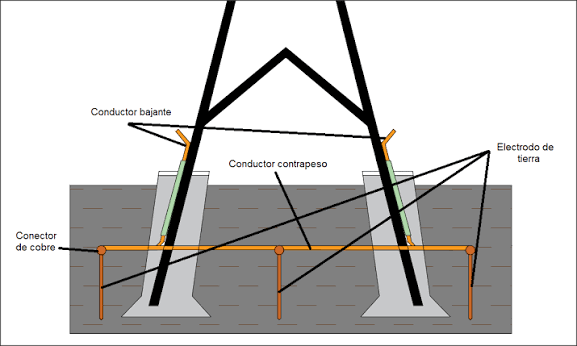
\includegraphics[width=0.45\textwidth]{Figs/Marco teorico/SPT.png}
    \caption{Configuración conceptual de un sistema de puesta a tierra con contrapesos horizontales y electrodos verticales.}
    \label{fig:spt_contrapesos}
\end{figure}


\subsection{Evaluación Estadística del Desempeño Atmosférico}

Para este propósito se emplean modelos estadísticos que combinan la actividad atmosférica de la zona, caracterizada mediante la densidad de descargas a tierra ($N_g$), con distribuciones probabilísticas asociadas a la magnitud de las corrientes de rayo. A partir de esta información es posible estimar la frecuencia de impactos sobre una línea y determinar la probabilidad de que dichos eventos produzcan la ruptura del aislamiento.

Uno de los indicadores más utilizados en estudios de desempeño atmosférico corresponde a la tasa de falla, expresada generalmente como el número esperado de eventos por cada 100 km de línea y por año. Este parámetro permite cuantificar el comportamiento de una estructura frente a descargas atmosféricas y comparar diferentes alternativas de diseño desde el punto de vista de la confiabilidad \cite{ieee1410}.



\subsubsection{Metodologías de Referencia para la Evaluación del Desempeño Atmosférico}

La evaluación probabilística de las tasas de salida en redes aéreas se fundamenta en los procedimientos estandarizados por el Instituto de Ingenieros Eléctricos y Electrónicos (\textsc{ieee}), los cuales diferencian el tratamiento metodológico según las características de la infraestructura:

\begin{itemize}
    \item \textbf{IEEE Std 1410:} Diseñada para líneas de distribución y subtransmisión \cite{ieee1410}. Establece los criterios para estimar la frecuencia de fallas considerando de forma rigurosa tanto impactos directos en conductores desprotegidos como sobretensiones inducidas por descargas indirectas cercanas a la servidumbre de la red de \SI{33}{\kV}.
    \item \textbf{IEEE Std 1243:} Orientada a líneas de transmisión con hilos de guarda \cite{IEEE_1243}. Proporciona los modelos probabilísticos para determinar la corriente crítica de falla y evaluar el mecanismo de \textit{Backflashover} (\textsc{bfo}) en función de la impedancia de impulso de las estructuras de soporte.
\end{itemize}


\section{Metodología}

\subsection{Datos generales del problema}
Para la evaluación del desempeño atmosférico se emplearon los parámetros eléctricos y ambientales suministrados para el grupo de estudio comprendido entre los apoyos A170 y A176. Estos parámetros permiten caracterizar tanto la actividad atmosférica de la zona como las condiciones eléctricas del terreno, constituyendo la información base para el modelado electromagnético y el análisis estadístico posterior.

La Tabla \ref{tab:datos_generales} resume los principales parámetros globales utilizados durante el desarrollo del proyecto.

\begin{table}[H]
\centering
\caption{Parámetros generales del caso de estudio.}
\label{tab:datos_generales}
\renewcommand{\arraystretch}{1.2}
\begin{tabular}{lc}
\toprule
Parámetro & Valor \\
\midrule
Nivel de tensión de la línea & 33 kV \\
Densidad de descargas a tierra ($N_g$) & 78.77 rayos/km$^2$/año \\
Corriente media de rayo ($I_{p,\mathrm{mean}}$) & 9.43 kA \\
Desviación estándar logarítmica ($\sigma$) & 0.65 \\
Corriente asociada al percentil 98 ($I_{98}$) & 35.8 kA \\
Frecuencia del sistema & 60 Hz \\
Radio del poste en la base (m) & 0.26 \\
Diámetro del poste en la cima (m) & 0.15 \\
Número de conductores de fase & 3  \\
Número de cables de guarda & 1 \\
\bottomrule
\end{tabular}
\end{table}

\subsection{Caracterización del nodo de estudio}

De acuerdo con la asignación establecida para el proyecto, el apoyo A173 fue seleccionado como nodo principal de estudio para el análisis del fenómeno de \textit{Backflashover} y el diseño del sistema de puesta a tierra. Debido a que las sobretensiones generadas por una descarga atmosférica se propagan a través de la línea en forma de ondas viajeras, fue necesario considerar también las estructuras adyacentes A172 y A174 con el fin de representar adecuadamente los fenómenos de reflexión y transmisión asociados a la propagación de dichas ondas.

La Tabla \ref{tab:nodos_estudio} presenta las principales características geométricas de las estructuras consideradas en el modelo detallado.

\begin{table}[H]
\centering
\caption{Características generales de las estructuras modeladas en detalle.}
\label{tab:nodos_estudio}
\renewcommand{\arraystretch}{1.2}
\begin{tabular}{lccc}
\toprule
Parámetro & A172 & A173 & A174 \\
\midrule
Tipo de estructura & Torre metálica & Tormenta R1 & Tormenta R1 \\
Longitud del vano (m) & 170.2 & 23.8 & 701.6 \\
Altura de fase, $Z_f$ (m) & 10.4 & 9.8 & 9.8 \\
Altura del cable de guarda, $Z_g$ (m) & 12.0 & 12.7 & 11.9 \\
Distancia efectiva de la cadena de aislamiento (cm) & 38.10 & 58.40 & 58.40 \\
\bottomrule
\end{tabular}
\end{table}

\subsection{Obtención de parámetros eléctricos de línea}

Se realizo la la obtención de los parámetros empleando el módulo \textit{Line Constants Program} (LCC) de ATP, utilizando como datos de entrada la configuración geométrica de los conductores de fase, el cable de guarda, las alturas de instalación y las longitudes de vano correspondientes a las estructuras comprendidas entre los apoyos A170 y A176. Adicionalmente, se incorporaron las características eléctricas de los conductores y las propiedades del terreno suministradas para el caso de estudio.

Las Tablas \ref{tab:geometria_posicion}  y \ref{tab:geometria_alturas} resumen los principales parámetros geométricos utilizados para la determinación de las constantes eléctricas de los diferentes tramos de línea. A partir de esta información se calcularon las matrices de parámetros distribuidos y las constantes modales necesarias para la construcción del modelo electromagnético en ATPDraw.

\begin{table}[H]
\centering
\caption{Posición geométrica de los conductores de fase y cable de guarda.}
\label{tab:geometria_posicion}
\renewcommand{\arraystretch}{1.2}
\begin{tabular}{ccccccc}
\toprule
Apoyo &
Longitud (m) &
$X_1$ (m) &
$X_2$ (m) &
$X_3$ (m) &
$X_G$ (m) \\
\midrule
A170 & 298.8 & -2.0 & 0.0 & 1.8 & 1.2 \\
A171 & 656.5 & -1.8 & 0.0 & 2.0 & -0.9 \\
A172 & 170.2 & -1.6 & 0.0 & 1.2 & -0.6 \\
A173 & 23.8  & -2.5 & 0.0 & 2.5 & 0.0 \\
A174 & 701.6 & -2.5 & 0.0 & 2.5 & 0.0 \\
A175 & 86.3  & -2.4 & 0.0 & 2.4 & 0.0 \\
A176 & 736.5 & -2.0 & 0.0 & 2.0 & -1.0 \\
\bottomrule
\end{tabular}
\end{table}
\begin{table}[H]
\centering
\caption{Alturas medias, flechas y resistividad del terreno para cada vano.}
\label{tab:geometria_alturas}
\renewcommand{\arraystretch}{1.2}
\begin{tabular}{cccccc}
\toprule
Apoyo &
$Z_f$ (m) &
$Z_G$ (m) &
$V_{mid}$ de las fases (m) &
$V_{mid}$ del guarda (m) &
$\rho$ ($\Omega\cdot$m) \\
\midrule
A170 & 12.0 & 16.2 & 10.80 & 15.39 & 350 \\
A171 & 12.5 & 14.5 & 11.34 & 13.78 & 317 \\
A172 & 10.4 & 12.0 & 9.45 & 11.40 & 349 \\
A173 & 9.8  & 12.7 & 9.00 & 12.07 & 420 \\
A174 & 9.8  & 11.9 & 9.00 & 11.31 & 388 \\
A175 & 11.8 & 14.2 & 10.80 & 13.49 & 448 \\
A176 & 12.7 & 15.8 & 11.70 & 15.01 & 246 \\
\bottomrule
\end{tabular}
\end{table}

\subsection{Determinación de impedancias de impulso de las estructuras}
Para acoplar la respuesta en alta frecuencia de las estructuras ante ondas de corriente de frente rápido, se adoptaron dos enfoques de modelado:
\begin{itemize}
    \item \textbf{Modelado Detallado (\textsc{A172}, \textsc{A173}, \textsc{A174}):} Representación segmentada de las bayonetas, crucetas y secciones del fuste vertical mediante líneas de transmisión en parámetros distribuidos. Las impedancias de onda individuales se determinaron analíticamente a partir de los radios equivalentes y alturas de cada componente estructural.
    \item \textbf{Modelado Simplificado (\textsc{A170}, \textsc{A171}, \textsc{A175}, \textsc{A176}):} Sustitución de los apoyos distantes por una impedancia concentrada equivalente de impulso.
\end{itemize}


\subsection{Diseño del sistema de puesta a tierra}

El proceso consideró la incorporación de contrapesos horizontales enterrados y electrodos verticales conectados a la estructura, utilizando como parámetros de entrada las características eléctricas del terreno y las restricciones de diseño establecidas en la guía del proyecto. Para cada alternativa evaluada se determinaron los parámetros eléctricos equivalentes del sistema de puesta a tierra mediante expresiones analíticas ampliamente utilizadas para el diseño de sistemas de dispersión de corriente de impulso.

La metodología de diseño se desarrolló de manera iterativa, modificando progresivamente la longitud, cantidad y disposición de los contrapesos horizontales, así como las características de los electrodos verticales. Para cada configuración se obtuvieron los parámetros requeridos para su implementación dentro del modelo electromagnético y para la posterior evaluación estadística del desempeño atmosférico.

Finalmente, las diferentes alternativas propuestas fueron comparadas mediante simulaciones electromagnéticas y análisis estadísticos, permitiendo identificar la configuración que proporcionó el mejor comportamiento frente a descargas atmosféricas para las condiciones del caso de estudio.

\subsection{Construcción del modelo electromagnético}

Una vez obtenidos los parámetros eléctricos de la línea, las impedancias de impulso de las estructuras y los parámetros asociados al sistema de puesta a tierra, se procedió a la construcción del modelo electromagnético en ATPDraw.

El modelo desarrollado incluyó la representación de los diferentes tramos de línea mediante parámetros distribuidos, las estructuras de soporte consideradas dentro del área de estudio, los sistemas de aislamiento y los elementos asociados a la puesta a tierra. Adicionalmente, se implementó una fuente de corriente de impulso para representar la descarga atmosférica, junto con los modelos requeridos para reproducir el comportamiento dinámico del aislamiento durante eventos transitorios.

Finalmente, se verificó la correcta integración de todos los elementos del modelo y se realizaron simulaciones preliminares para validar el comportamiento general de la red antes de proceder con la evaluación del desempeño atmosférico.

\subsection{Evaluación estadística del desempeño}

Una vez validado el modelo electromagnético, se realizó la evaluación estadística del desempeño atmosférico de la estructura de estudio mediante IEEE Flash 2.04.

Para esta etapa se emplearon como datos de entrada las características geométricas de la línea, los parámetros del aislamiento, las condiciones del sistema de puesta a tierra, la resistividad del terreno y los parámetros estadísticos asociados a la actividad atmosférica de la zona de estudio. Con esta información se estimaron los indicadores de desempeño necesarios para evaluar la susceptibilidad de la estructura frente al fenómeno de \textit{Backflashover}.

%------------------------------------------
\section{Herramientas de Software Utilizadas}

\subsection{ATPDraw}

\textsc{ATPDraw} se empleó como la plataforma principal para el modelado electromagnético y la simulación de transitorios en alta frecuencia. El programa resolvió de forma determinística las ecuaciones de onda ante el fenómeno de \textit{Backflashover}, integrando las matrices multifásicas distribuidas de la línea con las impedancias de onda segmentadas de los apoyos \cite{martinez2017power}.

Para representar la descarga atmosférica, se implementó una fuente de corriente impulsiva parametrizada mediante la función de Heidler en conjunto con una resistencia de $\SI{500}{\Omega}$ que modela la impedancia del canal del rayo (Figura~\ref{fig:atp_fuente_rayo}). Asimismo, la disrupción dieléctrica en las cadenas de aisladores se representó mediante el modelo dinámico \textit{Volt-Time} (Figura~\ref{fig:atp_volttime}), el cual gobierna la apertura o cierre de interruptores no lineales cuando la severidad del transitorio supera la curva de soportabilidad del aislamiento. Los sistemas de puesta a tierra se incorporaron mediante el acoplamiento de parámetros distribuidos para capturar de forma precisa el comportamiento inductivo inicial de los contrapesos.

\begin{figure}[htbp]
    \centering
    \begin{subfigure}[t]{0.35\textwidth}
        \centering
        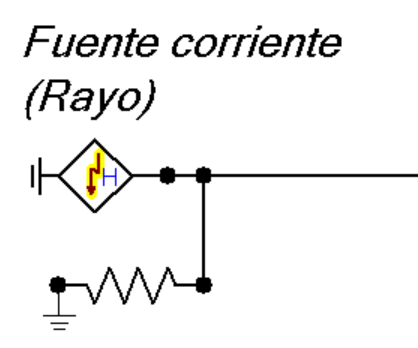
\includegraphics[width=\linewidth]{Figs/Herramientas/Rayos_source.png}
        \caption{Fuente de corriente impulsiva y resistencia de canal en \textsc{ATPDraw}.}
        \label{fig:atp_fuente_rayo}
    \end{subfigure}
    \hfill
    \begin{subfigure}[t]{0.35\textwidth}
        \centering
        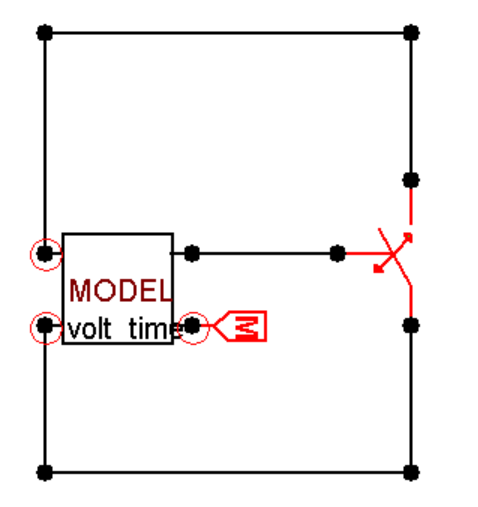
\includegraphics[width=\linewidth]{Figs/Herramientas/Volt_time.png}
        \caption{Modelo \textit{Volt-Time} para la ruptura dieléctrica del aislamiento.}
        \label{fig:atp_volttime}
    \end{subfigure}
    \caption{Elementos principales implementados en \textsc{ATPDraw} para la simulación del desempeño frente a descargas atmosféricas.}
    \label{fig:modelos_atp}
\end{figure} 

\subsection{\textsc{IEEE Flash 2.04}}
El software \textsc{IEEE Flash 2.04} se utilizó para automatizar la evaluación estadística y determinar la Tasa de Salidas de Línea (TFR) anual por cada \SI{100}{\km\text{-año}}. La herramienta procesó de forma agregada la actividad atmosférica local ($N_g$) y la caracterización geométrica del tramo bajo las directrices normativas de las guías IEEE Std 1243 e IEEE Std 1410 \cite{ieee1410}. Esto permitió discriminar probabilísticamente el riesgo de salidas de la infraestructura de \SI{33}{\kV} debido a fallas por apantallamiento (\textit{Shielding Failure}) y, críticamente en el nodo de estudio \textsc{A173}, fallas por contorneo inverso (\textit{Backflashover}).

\subsection{SMath Studio}
SMath Studio operó como el entorno de cálculo numérico para la programación, documentación y validación de las memorias de cálculo del proyecto. Su aplicación se concentró en la resolución analítica de las ecuaciones geométricas de las torres y en el diseño iterativo del sistema de puesta a tierra. El programa permitió determinar de forma dinámica las variaciones de la impedancia de impulso equivalente y el comportamiento no lineal del terreno al modificar paramétricamente la longitud efectiva de los contrapesos horizontales y la disposición de los electrodos verticales, consolidando la base de parámetros de entrada cargados en \textsc{ATPDraw}.

%----------------------------------------------

\section{Desarrollo del Modelo}

\subsection{Obtención de parámetros de línea}

Con el propósito de facilitar la extracción y presentación de los parámetros eléctricos obtenidos mediante LCC, se seleccionó la representación mediante modelo $\pi$ nominal. Esta elección no corresponde al modelo utilizado posteriormente en las simulaciones de transitorios electromagnéticos, sino únicamente a una configuración de cálculo que permite obtener de manera directa los parámetros modales de secuencia positiva y cero reportados por la herramienta.

La Figura~\ref{fig:lcc_icono} muestra el componente LCC utilizado dentro de ATPDraw para la caracterización de los diferentes tramos de línea, mientras que la Figura~\ref{fig:lcc_pi} presenta la configuración empleada para la obtención de los parámetros eléctricos mediante el modelo $\pi$ nominal.

\begin{figure}[H]
    \centering
    \begin{subfigure}[t]{0.22\textwidth}
        \centering
        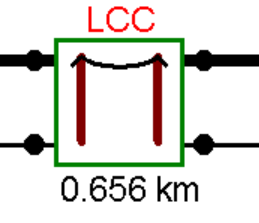
\includegraphics[width=0.8\linewidth]{Figs/Modelado/LCC.png}
        \caption{Componente \textit{Line Constants Program} (LCC).}
        \label{fig:lcc_icono}
    \end{subfigure}
    \hfill
    \begin{subfigure}[t]{0.4\textwidth}
        \centering
        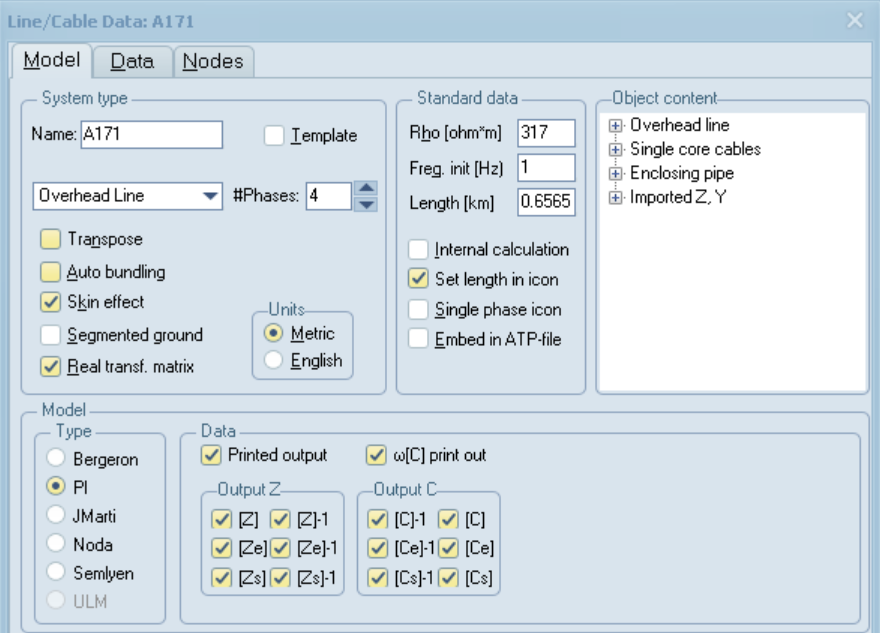
\includegraphics[width=\linewidth]{Figs/Modelado/Modelado.png}
        \caption{Configuración del módulo LCC empleando la representación mediante modelo $\pi$ nominal.}
        \label{fig:lcc_pi}
    \end{subfigure}
    \caption{Implementación del módulo \textit{Line Constants Program} (LCC) y configuración utilizada para el cálculo de los parámetros eléctricos de la línea.}
    \label{fig:lcc_modelado}
\end{figure}


Los resultados obtenidos mediante LCC se encuentran en las tablas \ref{tab:lcc_a170} - \ref{tab:lcc_a176}, en estas se incluyen la impedancia característica de propagación, la constante de atenuación, la velocidad de propagación de las ondas electromagnéticas y los parámetros distribuidos de resistencia, reactancia y susceptancia para las secuencias positiva y cero. Estos parámetros constituyen la base para la construcción del modelo electromagnético de la línea y permiten representar adecuadamente los fenómenos de propagación asociados a descargas atmosféricas.

\begin{table}[H]
\centering
\caption{Parámetros modales de la línea asociados al apoyo A170.}
\label{tab:lcc_a170}
\renewcommand{\arraystretch}{1.2}
\begin{tabular}{lccccccc}
\toprule
Secuencia &
$\left|Z_s\right|$ ($\Omega$) &
$\angle Z_s$ ($^\circ$) &
$\alpha$ (dB/km) &
$v$ (km/s) &
$R$ ($\Omega$/km) &
$X$ ($\Omega$/km) &
$B$ (mho/km) \\
\midrule
Cero     & 3688.61 & -42.17 & $6.4169\times10^{-4}$ & 77028.3 & 0.403955 & 0.040081 & $2.9836\times10^{-8}$ \\
Positiva & 2622.92 & -44.44 & $9.2993\times10^{-4}$ & 57549.5 & 0.401000 & 0.007852 & $5.8299\times10^{-8}$ \\
\bottomrule
\end{tabular}
\end{table}
\begin{table}[H]
\centering
\caption{Parámetros modales de la línea asociados al apoyo A171.}
\label{tab:lcc_a171}
\renewcommand{\arraystretch}{1.2}
\begin{tabular}{lccccccc}
\toprule
Secuencia &
$\left|Z_s\right|$ ($\Omega$) &
$\angle Z_s$ ($^\circ$) &
$\alpha$ (dB/km) &
$v$ (km/s) &
$R$ ($\Omega$/km) &
$X$ ($\Omega$/km) &
$B$ (mho/km) \\
\midrule
Cero     & 3596.99 & -42.18 & $6.5817\times10^{-4}$ & 75134.0 & 0.403954 & 0.039895 & $3.1373\times10^{-8}$ \\
Positiva & 2622.23 & -44.44 & $9.3017\times10^{-4}$ & 57534.4 & 0.401000 & 0.007852 & $5.8329\times10^{-8}$ \\
\bottomrule
\end{tabular}
\end{table}
\begin{table}[H]
\centering
\caption{Parámetros modales de la línea asociados al apoyo A172.}
\label{tab:lcc_a172}
\renewcommand{\arraystretch}{1.2}
\begin{tabular}{lccccccc}
\toprule
Secuencia &
$\left|Z_s\right|$ ($\Omega$) &
$\angle Z_s$ ($^\circ$) &
$\alpha$ (dB/km) &
$v$ (km/s) &
$R$ ($\Omega$/km) &
$X$ ($\Omega$/km) &
$B$ (mho/km) \\
\midrule
Cero     & 3582.72 & -42.11 & $6.6008\times10^{-4}$ & 74738.3 & 0.403956 & 0.040858 & $3.1631\times10^{-8}$ \\
Positiva & 2552.31 & -44.47 & $9.5611\times10^{-4}$ & 56028.2 & 0.401000 & 0.007461 & $6.1568\times10^{-8}$ \\
\bottomrule
\end{tabular}
\end{table}

\begin{table}[H]
\centering
\caption{Parámetros modales de la línea asociados al apoyo A173.}
\label{tab:lcc_a173}
\renewcommand{\arraystretch}{1.2}
\begin{tabular}{lccccccc}
\toprule
Secuencia &
$\left|Z_s\right|$ ($\Omega$) &
$\angle Z_s$ ($^\circ$) &
$\alpha$ (dB/km) &
$v$ (km/s) &
$R$ ($\Omega$/km) &
$X$ ($\Omega$/km) &
$B$ (mho/km) \\
\midrule
Cero     & 3489.96 & -42.19 & $6.7848\times10^{-4}$ & 72914.2 & 0.403956 & 0.039732 & $3.3326\times10^{-8}$ \\
Positiva & 2680.92 & -44.41 & $9.0942\times10^{-4}$ & 58796.3 & 0.401000 & 0.008198 & $5.5804\times10^{-8}$ \\
\bottomrule
\end{tabular}
\end{table}

\begin{table}[H]
\centering
\caption{Parámetros modales de la línea asociados al apoyo A174.}
\label{tab:lcc_a174}
\renewcommand{\arraystretch}{1.2}
\begin{tabular}{lccccccc}
\toprule
Secuencia &
$\left|Z_s\right|$ ($\Omega$) &
$\angle Z_s$ ($^\circ$) &
$\alpha$ (dB/km) &
$v$ (km/s) &
$R$ ($\Omega$/km) &
$X$ ($\Omega$/km) &
$B$ (mho/km) \\
\midrule
Cero     & 3450.98 & -42.20 & $6.8622\times10^{-4}$ & 72109.6 & 0.403956 & 0.039630 & $3.4082\times10^{-8}$ \\
Positiva & 2680.25 & -44.41 & $9.0965\times10^{-4}$ & 58781.7 & 0.401000 & 0.008198 & $5.5832\times10^{-8}$ \\
\bottomrule
\end{tabular}
\end{table}

\begin{table}[H]
\centering
\caption{Parámetros modales de la línea asociados al apoyo A175.}
\label{tab:lcc_a175}
\renewcommand{\arraystretch}{1.2}
\begin{tabular}{lccccccc}
\toprule
Secuencia &
$\left|Z_s\right|$ ($\Omega$) &
$\angle Z_s$ ($^\circ$) &
$\alpha$ (dB/km) &
$v$ (km/s) &
$R$ ($\Omega$/km) &
$X$ ($\Omega$/km) &
$B$ (mho/km) \\
\midrule
Cero     & 3506.60 & -42.18 & $6.7509\times10^{-4}$ & 73239.7 & 0.403955 & 0.039957 & $3.3012\times10^{-8}$ \\
Positiva & 2672.36 & -44.42 & $9.1240\times10^{-4}$ & 58612.3 & 0.401000 & 0.008147 & $5.6162\times10^{-8}$ \\
\bottomrule
\end{tabular}
\end{table}

\begin{table}[H]
\centering
\caption{Parámetros modales de la línea asociados al apoyo A176.}
\label{tab:lcc_a176}
\renewcommand{\arraystretch}{1.2}
\begin{tabular}{lccccccc}
\toprule
Secuencia &
$\left|Z_s\right|$ ($\Omega$) &
$\angle Z_s$ ($^\circ$) &
$\alpha$ (dB/km) &
$v$ (km/s) &
$R$ ($\Omega$/km) &
$X$ ($\Omega$/km) &
$B$ (mho/km) \\
\midrule
Cero     & 3646.45 & -42.15 & $6.4891\times10^{-4}$ & 76119.5 & 0.403955 & 0.040355 & $3.0532\times10^{-8}$ \\
Positiva & 2634.40 & -44.43 & $9.2580\times10^{-4}$ & 57796.6 & 0.401000 & 0.007918 & $5.7792\times10^{-8}$ \\
\bottomrule
\end{tabular}
\end{table}

\subsection{Cálculo de impedancias de los apoyos}

Con el propósito de representar adecuadamente estos fenómenos en el modelo electromagnético, se determinaron las impedancias de impulso y los tiempos de propagación asociados a las estructuras comprendidas dentro del tramo de estudio. Debido a las diferencias constructivas existentes entre los apoyos analizados, se adoptaron dos estrategias de modelado: una representación detallada para las estructuras involucradas directamente en el análisis del fenómeno de \textit{Backflashover} y una representación simplificada para los apoyos restantes.

\subsubsection{Modelos detallados de alta frecuencia}

\paragraph{Nodo A172}

El nodo A172 corresponde a una torre metálica cuya impedancia de impulso fue calculada mediante:

\begin{equation}
Z_{eq,A172}
=
60\ln
\left(
\sqrt{2}
\sqrt{
\left(\frac{H}{r}\right)^2+1
}
\right)
\end{equation}

considerando una altura total de:

\begin{equation*}
H=10.5\ \mathrm{m}
\end{equation*}

y un radio equivalente en la base de:

\begin{equation*}
r=0.26\ \mathrm{m}
\end{equation*}

obteniéndose:

\begin{equation*}
Z_{eq,A172}=242.72\ \Omega
\end{equation*}

El tiempo de propagación asociado se determinó mediante:

\begin{equation*}
\tau=\frac{H}{c}
\end{equation*}

resultando:

\begin{equation*}
\tau_{A172}=3.50\times10^{-8}\ \mathrm{s}
\end{equation*}


\paragraph{Nodos A173 y A174:}

Para las estructuras tipo Tormenta R1 (A173 y A174), la impedancia característica de cada uno de los tres montantes principales fue calculada mediante:

\begin{equation}
Z_1=
60\ln
\left(
\frac{\sqrt{2}H}
{\sqrt[3]{D_{12}D_{13}r}}
\right)
\end{equation}

\begin{equation}
Z_2=
60\ln
\left(
\frac{\sqrt{2}H}
{\sqrt[3]{D_{12}D_{23}r}}
\right)
\end{equation}

\begin{equation}
Z_3=
60\ln
\left(
\frac{\sqrt{2}H}
{\sqrt[3]{D_{13}D_{23}r}}
\right)
\end{equation}

donde:

\begin{equation*}
H=10\ \mathrm{m}
\end{equation*}

\begin{equation*}
D_{12}=D_{13}=D_{23}=0.15\ \mathrm{m}
\end{equation*}

\begin{equation*}
r=0.26\ \mathrm{m}
\end{equation*}

obteniéndose:

\begin{equation*}
Z_1=Z_2=Z_3=261.78\ \Omega
\end{equation*}

La impedancia equivalente del cuerpo principal resulta:

\begin{equation*}
Z_{eq}
=
\left(
\frac{1}{Z_1}
+
\frac{1}{Z_2}
+
\frac{1}{Z_3}
\right)^{-1}
=
87.26\ \Omega
\end{equation*}

El tiempo de propagación asociado se calculó mediante:

\begin{equation*}
\tau=
\frac{H}{0.85c}
=3.92\times10^{-8}\ \mathrm{s}
\end{equation*}

\subsubsection{Calculo de crucetas y bayonetas}

Para las crucetas y bayonetas fue necesario determinar previamente las dimensiones geométricas asociadas a cada elemento estructural. Estas dimensiones se obtuvieron a partir de la posición horizontal de las fases y del cable de guarda mostradas en la Tabla~\ref{tab:geometria_posicion}, así como de las alturas indicadas en la Tabla~\ref{tab:geometria_alturas}.

En las se consideraron tres segmentos horizontales equivalentes denominados AB, BN y NC. El segmento AB corresponde a la distancia horizontal entre la fase A y la fase B, el segmento BN representa la distancia entre la fase B y el cable de guarda, mientras que el segmento NC corresponde a la distancia horizontal entre el cable de guarda y la fase C.

Las longitudes de estos segmentos se determinaron mediante:

\begin{equation}
h_{AB}=|X_2-X_1|
\end{equation}

\begin{equation}
h_{BN}=|X_G-X_2|
\end{equation}

\begin{equation}
h_{NC}=|X_3-X_G|
\end{equation}

La longitud de la bayoneta se calculó a partir de la diferencia entre la altura del cable de guarda y la altura total de la estructura:

\begin{equation}
h_{BAY}=Z_G-H
\end{equation}


Las impedancias de las crucetas y bayonetas se calcularon mediante:

\begin{equation}
Z=
60\ln
\left(
\frac{\pi h}
{\exp(L+y)}
\right)
\end{equation}

considerando:

\begin{equation}
L=0.05\ \mathrm{m}
\end{equation}

\begin{equation}
y=0.004\ \mathrm{m}
\end{equation}

Los tiempos de tránsito asociados se determinaron mediante:

\begin{equation}
\tau=
\frac{h}{0.8c}
\end{equation}

Los parámetros calculados para las crucetas y bayonetas de los apoyos modelados en detalle se resumen en la Tabla~\ref{tab:crucetas_detalladas}.

\begin{table}[H]
\centering
\caption{Parámetros calculados para crucetas y bayonetas de los apoyos modelados en detalle.}
\label{tab:crucetas_detalladas}
\renewcommand{\arraystretch}{1.2}
\begin{tabular}{lcccc}
\toprule
Apoyo & Elemento & $h$ (m) & $Z$ ($\Omega$) & $\tau$ (s) \\
\midrule
A172 & Cruceta AB & 1.6 & 93.644 & $6.6713\times10^{-9}$ \\
A172 & Cruceta BN & 0.6 & 34.79 & $2.50\times10^{-9}$ \\
A172 & Cruceta CN & 0.6 & 34.79 & $2.50\times10^{-9}$ \\
A172 & Bayoneta & 1.5 & 89.7717 & $6.2543\times10^{-9}$ \\
A173 & Cruceta AB & 2.5 & 120.42 & $1.04\times10^{-8}$ \\
A173 & Cruceta BN & 0.0 & 0.00 & 0.00 \\
A173 & Cruceta NC & 2.5 & 120.42 & $1.04\times10^{-8}$ \\
A173 & Bayoneta & 2.7 & 125.04 & $1.13\times10^{-8}$ \\
A174 & Cruceta AB & 2.5 & 120.42 & $1.04\times10^{-8}$ \\
A174 & Cruceta BN & 0.0 & 0.00 & 0.00 \\
A174 & Cruceta NC & 2.5 & 120.42 & $1.04\times10^{-8}$ \\
A174 & Bayoneta & 1.9 & 103.96 & $7.92\times10^{-9}$ \\
\bottomrule
\end{tabular}
\end{table}

Se puede observar que el tramo BN para el nodo A173 y A174, presenta longitud nula debido a que la fase central y el cable de guarda se encuentran alineados verticalmente sobre el mismo eje de la estructura. Por esta razón, dicho tramo no aporta impedancia ni tiempo de propagación al modelo.

\subsubsection{Modelos simplificados equivalentes}

Las estructuras A170, A171, A175 y A176 fueron representadas mediante modelos equivalentes simplificados. 

Para las estructuras A170,A171,A176 debido a que trata de postes tipo H, se empleó una representación equivalente basada en dos montantes conectados en paralelo, cuya impedancia característica se determinó mediante:

\begin{equation}
Z=
60\ln
\left(
\sqrt{2}
\sqrt{
\left(
\frac{H}{r}
\right)^2+1
}
\right)
\end{equation}

donde:

\begin{itemize}
\item $H$ corresponde a la altura total de la estructura.
\item $r$ corresponde al radio equivalente en la base del apoyo.
\end{itemize}

La impedancia equivalente del modelo se obtuvo mediante:

\begin{equation}
Z_{eq}=\frac{Z_1 Z_2}
{Z_1+Z_2}
\end{equation}

considerando que ambos montantes presentan las mismas características geométricas, por lo que:

\begin{equation}
Z_1=Z_2=Z
\end{equation}

El tiempo de propagación asociado se calculó mediante:

\begin{equation}
\tau=
\frac{H}{c}
\end{equation}

donde (c) corresponde a la velocidad de la luz.

\paragraph{Nodo A170}

Para el nodo A170 se consideró:

\begin{equation*}
H=12\ \mathrm{m}
\end{equation*}

\begin{equation*}
r=0.35\ \mathrm{m}
\end{equation*}

obteniéndose:

\begin{equation*}
Z_1=Z_2=250.72\ \Omega
\end{equation*}

\begin{equation*}
Z_{eq,A170}=125.36\ \Omega
\end{equation*}

\begin{equation*}
\tau_{A170}
=4.00\times10^{-8}\ \mathrm{s}
\end{equation*}

\paragraph{Nodo A171:}

Para el apoyo Nodo se consideró:

\begin{equation*}
H=12.5\ \mathrm{m}
\end{equation*}

\begin{equation*}
r=0.35\ \mathrm{m}
\end{equation*}

obteniéndose:

\begin{equation*}
Z_1=Z_2=253.66\ \Omega
\end{equation*}

\begin{equation*}
Z_{eq,A171}=126.83\ \Omega
\end{equation*}

\begin{equation*}
\tau_{A171}=4.17\times10^{-8}\ \mathrm{s}
\end{equation*}

\paragraph{Nodo A175}

Para las estructuras tipo Tormenta R1 (A175), la impedancia característica de cada uno de los tres montantes principales fue calculada mediante:

\begin{equation*}
H=12\ \mathrm{m}
\end{equation*}

\begin{equation*}
D_{12}=D_{13}=D_{23}=0.15\ \mathrm{m}
\end{equation*}

\begin{equation*}
r=0.26\ \mathrm{m}
\end{equation*}

obteniéndose:

\begin{equation*}
Z_1=Z_2=Z_3=272.7151\ \Omega
\end{equation*}

La impedancia equivalente del cuerpo principal resulta:

\begin{equation*}
Z_{eq}
=
\left(
\frac{1}{Z_1}
+
\frac{1}{Z_2}
+
\frac{1}{Z_3}
\right)^{-1}
=
90.905\ \Omega
\end{equation*}

El tiempo de propagación asociado se calculó mediante:

\begin{equation*}
\tau=
\frac{H}{0.85c}
=4.7091\times10^{-8}\ \mathrm{s}
\end{equation*}
\paragraph{Nodo A176}

Para el nodo A176 se consideró:

\begin{equation*}
H=12.7\ \mathrm{m}
\end{equation*}

\begin{equation*}
r=0.35\ \mathrm{m}
\end{equation*}

obteniéndose:

\begin{equation*}
Z_1=Z_2=255.52\ \Omega
\end{equation*}

\begin{equation*}
Z_{eq,A176}
=127.76\ \Omega
\end{equation*}

\begin{equation*}
\tau_{A176} =4.23\times10^{-8}\ \mathrm{s}
\end{equation*}

La Tabla \ref{tab:modelos_simplificados} resume los resultados del los modelos simplificados:

\begin{table}[H]
\centering
\caption{Parámetros obtenidos para los apoyos modelados mediante representaciones simplificadas.}
\label{tab:modelos_simplificados}
\renewcommand{\arraystretch}{1.2}
\begin{tabular}{lccc}
\toprule
Apoyo & $Z_{eq}$ ($\Omega$) & $Z_{eq}$ ($\Omega$) & $\tau$ (s) \\
\midrule
A170 & 250.72 & 125.36 & $4.00\times10^{-8}$ \\
A171 & 253.66 & 126.83 & $4.17\times10^{-8}$ \\
A175 & 181.82 & 90.91 & $3.93\times10^{-8}$ \\
A176 & 255.52 & 127.76 & $4.23\times10^{-8}$ \\
\bottomrule
\end{tabular}
\end{table}

\subsection{Modelado de los aisladores}

Las cadenas de aislamiento de las estructuras modeladas fueron representadas mediante un circuito equivalente compuesto por una capacitancia concentrada y un modelo dinámico de ruptura dieléctrica, tal como se muestra en la Figura \ref{fig:modelo_aislador}.

El modelo implementado considera dos fenómenos fundamentales. En primer lugar, la capacitancia equivalente de la cadena de aisladores permite representar el comportamiento electrostático asociado a la distribución de cargas durante la propagación de las sobretensiones atmosféricas. Para este estudio se adoptó una capacitancia equivalente de:

\begin{equation}
C_{ais}=2.5\times10^{-6}\ \mathrm{F}
\end{equation}

valor utilizado en todos los apoyos modelados.

En segundo lugar, la evaluación de la ruptura dieléctrica fue realizada mediante el componente \texttt{GRP} de ATPDraw, configurado para implementar el criterio \textit{Volt-Time} descrito previamente en el marco teórico. Este modelo compara continuamente la tensión desarrollada sobre la cadena de aislamiento con la característica de soportabilidad definida para la estructura. Cuando la solicitación supera el límite establecido por la curva Volt-Time, el modelo conmuta automáticamente a un estado conductor, representando la ocurrencia de un fenómeno de \textit{Flashover} o \textit{Backflashover}.

La parametrización del modelo Volt-Time requiere como dato principal la distancia efectiva total de la cadena de aislamiento, la cual depende de la configuración geométrica de cada apoyo. Este parámetro determina el nivel de soportabilidad al impulso de la cadena y constituye una de las variables fundamentales en la evaluación del desempeño atmosférico de la línea.

Para los este modelado se emplearon las distancias efectivas de aislamiento resumidas en la Tabla \ref{tab:nodos_estudio}.

La combinación del modelo capacitivo con el bloque Volt-Time permitió reproducir de forma realista la respuesta dinámica del aislamiento frente a las sobretensiones originadas por descargas atmosféricas, posibilitando la identificación automática de eventos de ruptura durante las simulaciones transitorias realizadas en ATPDraw.

\begin{figure}[H]
\centering
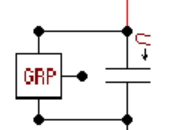
\includegraphics[width=0.28\textwidth]{Figs/Modelado/Aislador.png}
\caption{Modelo equivalente de la cadena de aislamiento implementado en ATPDraw mediante una capacitancia concentrada y un bloque \textit{Volt-Time}.}
\label{fig:modelo_aislador}
\end{figure}

\subsection{Modelado de los apoyos}

Una vez determinadas las impedancias de impulso y los tiempos de propagación asociados a los diferentes elementos estructurales, se procedió a la implementación de los apoyos en ATPDraw. Para las estructuras A172, A173 y A174 se utilizaron modelos detallados de alta frecuencia que permiten representar explícitamente la propagación de las ondas transitorias a través de los diferentes componentes de la estructura.

En el caso del apoyo A172, correspondiente a una torre metálica, el modelo incorpora la impedancia característica del cuerpo principal de la estructura y las impedancias asociadas a las crucetas. Por su parte, los apoyos A173 y A174 fueron representados mediante modelos de tres montantes, incluyendo además las impedancias de las crucetas y bayonetas calculadas a partir de la geometría de las estructuras tipo Tormenta R1.

La Figura \ref{fig:modelos_detallados} presenta la implementación final de los apoyos A172, A173 y A174 dentro del modelo electromagnético desarrollado en ATPDraw.

\begin{figure}[H]
\centering

\begin{subfigure}[b]{0.32\textwidth}
    \centering
    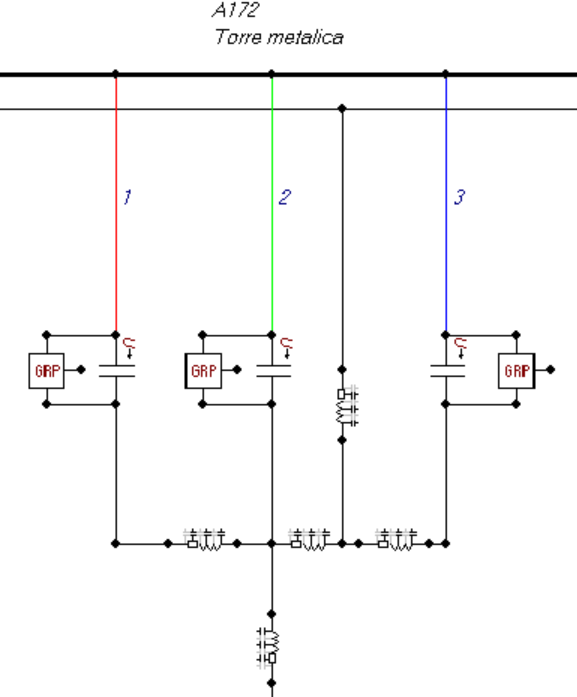
\includegraphics[width=\textwidth]{Figs/Modelado/A172.png}
    \caption{Modelo detallado del apoyo A172.}
    \label{fig:modelo_a172}
\end{subfigure}
\hfill
\begin{subfigure}[b]{0.32\textwidth}
    \centering
    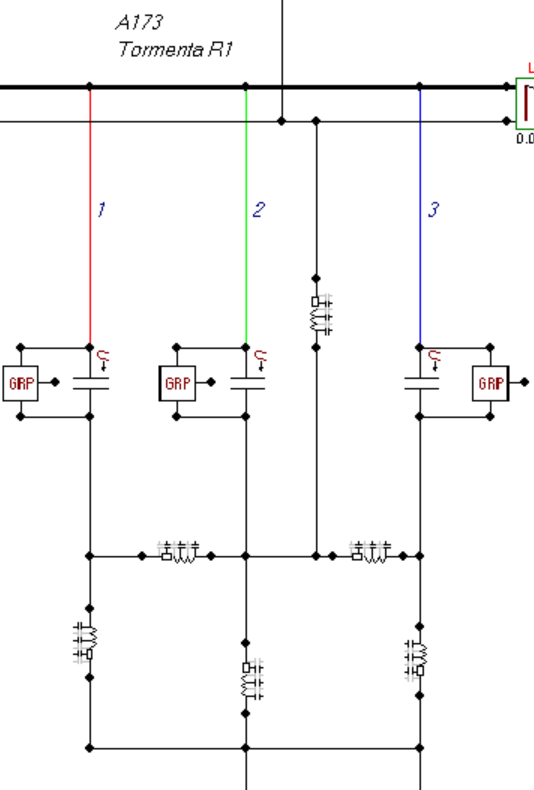
\includegraphics[width=\textwidth]{Figs/Modelado/A173.png}
    \caption{Modelo detallado del apoyo A173.}
    \label{fig:modelo_a173}
\end{subfigure}
\hfill
\begin{subfigure}[b]{0.32\textwidth}
    \centering
    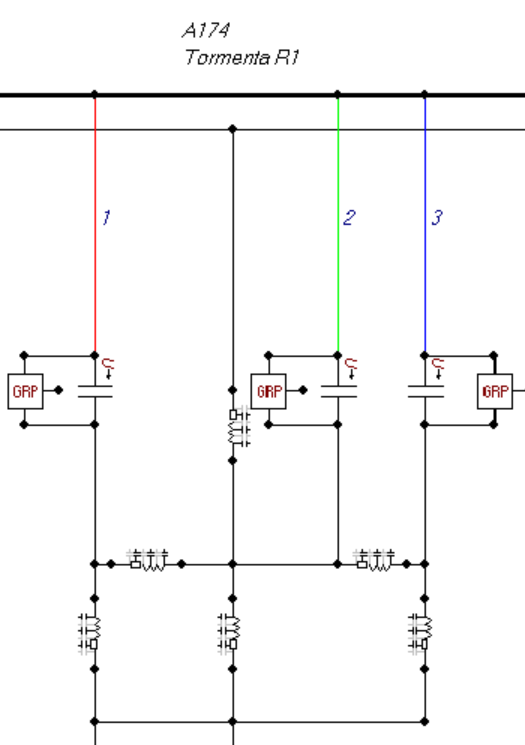
\includegraphics[width=\textwidth]{Figs/Modelado/A174.png}
    \caption{Modelo detallado del apoyo A174.}
    \label{fig:modelo_a174}
\end{subfigure}

\caption{Implementación en ATPDraw de los apoyos modelados mediante representaciones detalladas de alta frecuencia.}
\label{fig:modelos_detallados}
\end{figure}



\section{Diseño del Sistema de Puesta a Tierra}

\subsection{Configuración inicial}

Como punto de partida para el proceso de diseño, se evaluó el comportamiento del nodo de estudio bajo una condición inicial sin la incorporación de contrapesos horizontales ni electrodos verticales adicionales. Esta configuración permitió identificar la respuesta natural de la estructura frente a una descarga atmosférica y verificar la necesidad de implementar mejoras en el sistema de puesta a tierra.

Los resultados obtenidos evidenciaron la ocurrencia de un fenómeno de \textit{Backflashover} (BFO), identificado mediante la activación del modelo Volt-Time implementado en ATPDraw. La elevada corriente impulsiva produjo un incremento significativo del potencial de la estructura, generando una diferencia de potencial suficiente para superar la capacidad de soportabilidad del aislamiento.

La Figura~\ref{fig:bfo_inicial} presenta la tensión registrada sobre una de las cadenas de aislamiento durante la simulación de la configuración inicial.

\begin{figure}[H]
\centering
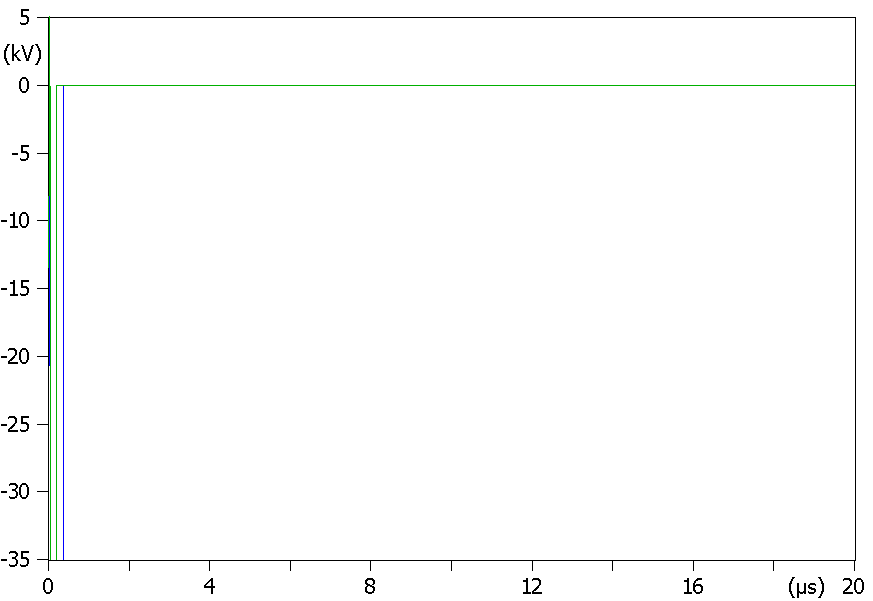
\includegraphics[width=0.65\textwidth]{Figs/Resultados/BFO1.png}
\caption{Respuesta del aislamiento para la configuración inicial sin optimización del sistema de puesta a tierra.}
\label{fig:bfo_inicial}
\end{figure}

La rápida variación de la tensión y la posterior actuación del modelo Volt-Time confirman la presencia de una falla por flameo inverso. Este resultado demuestra que la configuración inicial no proporciona una trayectoria de baja impedancia suficiente para disipar adecuadamente la corriente de rayo hacia el terreno.

A partir de esta observación se planteó el diseño de elementos adicionales de puesta a tierra, incluyendo contrapesos horizontales y electrodos verticales, con el propósito de reducir la elevación de potencial de la estructura y mejorar el desempeño atmosférico del sistema.


\subsection{Diseño de electrodos verticales}

Con el fin de mejorar la disipación de la corriente impulsiva hacia el terreno, se incorporaron electrodos verticales al sistema de puesta a tierra. Para el diseño de estos elementos se empleó la resistividad correspondiente al nodo principal de estudio, dada por:

\begin{equation}
\rho=420\ \Omega\cdot m
\end{equation}

Este valor corresponde a la resistividad del terreno asociada al apoyo A173 y fue utilizado para la obtención de los parámetros eléctricos implementados posteriormente en ATPDraw.

Los electrodos fueron representados mediante un modelo distribuido equivalente, considerando una longitud:

\begin{equation*}
l=2.4\ \mathrm{m}
\end{equation*}

un radio de conductor:

\begin{equation*}
a=0.005\ \mathrm{m}
\end{equation*}


Asimismo, se emplearon los valores:

\begin{equation*}
\varepsilon=8.8542\times10^{-12}\ \mathrm{F/m}
\end{equation*}

\begin{equation*}
\mu=4\pi\times10^{-7}\ \mathrm{H/m}
\end{equation*}

La resistencia distribuida asociada al electrodo vertical se calculó mediante:

\begin{equation}
R_i=
\frac{\rho}{2\pi}
\frac{n}{l}
\left(
\ln
\left(
\frac{4l}{a}
\right)
-1
\right)
\label{eq:r_varilla}
\end{equation}

obteniéndose:

\begin{equation*}
R_i=182.7121\ \Omega
\end{equation*}

La inductancia distribuida se determinó mediante:

\begin{equation}
L_i=
\frac{\mu}{2\pi}
\frac{l}{n}
\left(
\ln
\left(
\frac{4l}{a}
\right)
-1
\right)
\label{eq:l_varilla}
\end{equation}

resultando:

\begin{equation*}
L_i=3.1488\times10^{-6}\ \mathrm{H}
\end{equation*}

Por su parte, la capacitancia distribuida fue calculada mediante:

\begin{equation}
C_i=
2\pi\varepsilon
\frac{l}{n}
\left(
\ln
\left(
\frac{4l}{a}
\right)
-1
\right)
\label{eq:c_varilla}
\end{equation}

obteniéndose:

\begin{equation*}
C_i=8.7589\times10^{-10}\ \mathrm{F}
\end{equation*}

Los parámetros calculados fueron posteriormente utilizados para la implementación del modelo distribuido de los electrodos verticales en ATPDraw, permitiendo representar de forma adecuada el comportamiento transitorio del sistema de puesta a tierra frente a corrientes impulsivas de origen atmosférico.

\begin{table}[H]
\centering
\caption{Parámetros distribuidos obtenidos para los electrodos verticales.}
\label{tab:parametros_varillas}
\renewcommand{\arraystretch}{1.2}
\begin{tabular}{cccc}
\toprule
$R_i$ ($\Omega$) & $L_i$ (H) & $C_i$ (F) & $\rho$ ($\Omega\cdot$m) \\
\midrule
182.7121 & $3.1488\times10^{-6}$ & $8.7589\times10^{-10}$ & 420 \\
\bottomrule
\end{tabular}
\end{table}

\subsection{Diseño de contrapesos}

Con el propósito de reducir la elevación de potencial de la estructura durante la circulación de corrientes impulsivas de rayo, se evaluaron diferentes longitudes de contrapeso horizontal conectadas al sistema de puesta a tierra. Para todas las configuraciones se mantuvo la resistividad correspondiente al nodo de estudio:

\begin{equation*}
\rho = 420\ \Omega\cdot m
\end{equation*}

así como un radio de conductor:

\begin{equation*}
a = 0.005\ \mathrm{m}
\end{equation*}

La evaluación se realizó de forma iterativa comenzando con una longitud de 40 m y reduciendo progresivamente el contrapeso hasta identificar la configuración mínima capaz de evitar la ocurrencia de fenómenos de \textit{Backflashover}.

\subsubsection{Contrapeso horizontal de 40 m}

Como primera alternativa se evaluó un contrapeso horizontal con una longitud total de:

\begin{equation*}
l=40\ \mathrm{m}
\end{equation*}

Para la discretización del modelo distribuido se emplearon:

\begin{equation*}
n=20
\end{equation*}

segmentos equivalentes.

La resistencia distribuida asociada a cada segmento fue calculada mediante:

\begin{equation}
R_i=
\frac{\rho}{2\pi}
\frac{n}{l}
\left(
\ln
\left(
\frac{4l}{a}
\right)-1
\right)
\label{eq:r40}
\end{equation}

obteniéndose:

\begin{equation*}
R_i=313.2859\ \Omega
\end{equation*}

La inductancia distribuida se determinó mediante:

\begin{equation}
L_i=
\frac{\mu}{2\pi}
\frac{l}{n}
\left(
\ln
\left(
\frac{4l}{a}
\right)-1
\right)
\label{eq:l40}
\end{equation}

resultando:

\begin{equation*}
L_i=3.7494\times10^{-6}\ \mathrm{H}
\end{equation*}

La capacitancia distribuida se calculó mediante:

\begin{equation}
C_i=
2\pi\varepsilon
\frac{l}{n}
\left(
\ln
\left(
\frac{4l}{a}
\right)-1
\right)
\label{eq:c40}
\end{equation}

obteniéndose:

\begin{equation*}
C_i=1.0429\times10^{-9}\ \mathrm{F}
\end{equation*}

Los resultados obtenidos para esta configuración se presentan en las Figuras~\ref{fig:contrapeso40_res1} y \ref{fig:contrapeso40_res2}. Se observa que, aunque la descarga atmosférica genera oscilaciones transitorias importantes durante los primeros instantes de la simulación, las tensiones desarrolladas sobre las cadenas de aislamiento permanecen dentro de la región de soportabilidad definida por el modelo Volt-Time.

En consecuencia, para esta configuración no se presentó la ocurrencia de fenómenos de \textit{Backflashover}, evidenciando que la longitud de 40 m proporciona una trayectoria de baja impedancia adecuada para la disipación de la corriente impulsiva hacia el terreno.

\begin{figure}[H]
    \centering

    \begin{subfigure}[t]{0.48\textwidth}
        \centering
        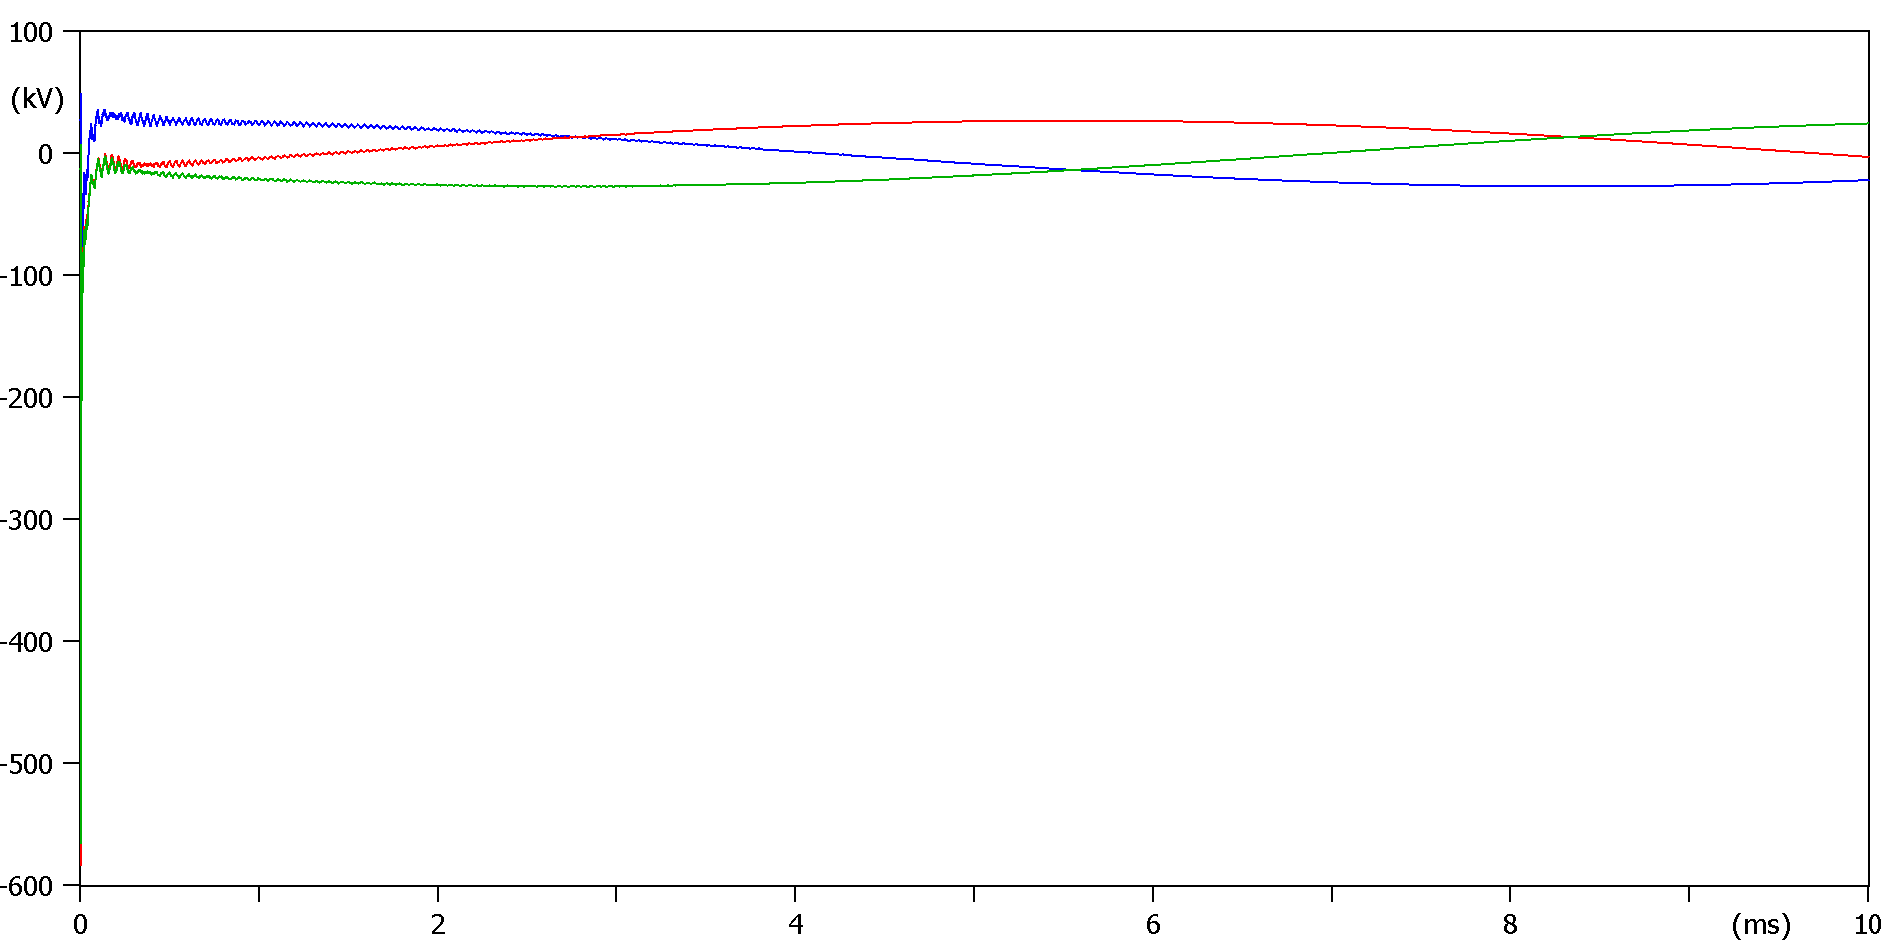
\includegraphics[width=\linewidth]{Figs/Resultados/40m_1.png}
        \caption{Respuesta temporal de las tensiones de fase para el contrapeso horizontal de 40 m.}
        \label{fig:contrapeso40_res1}
    \end{subfigure}
    \hfill
    \begin{subfigure}[t]{0.48\textwidth}
        \centering
        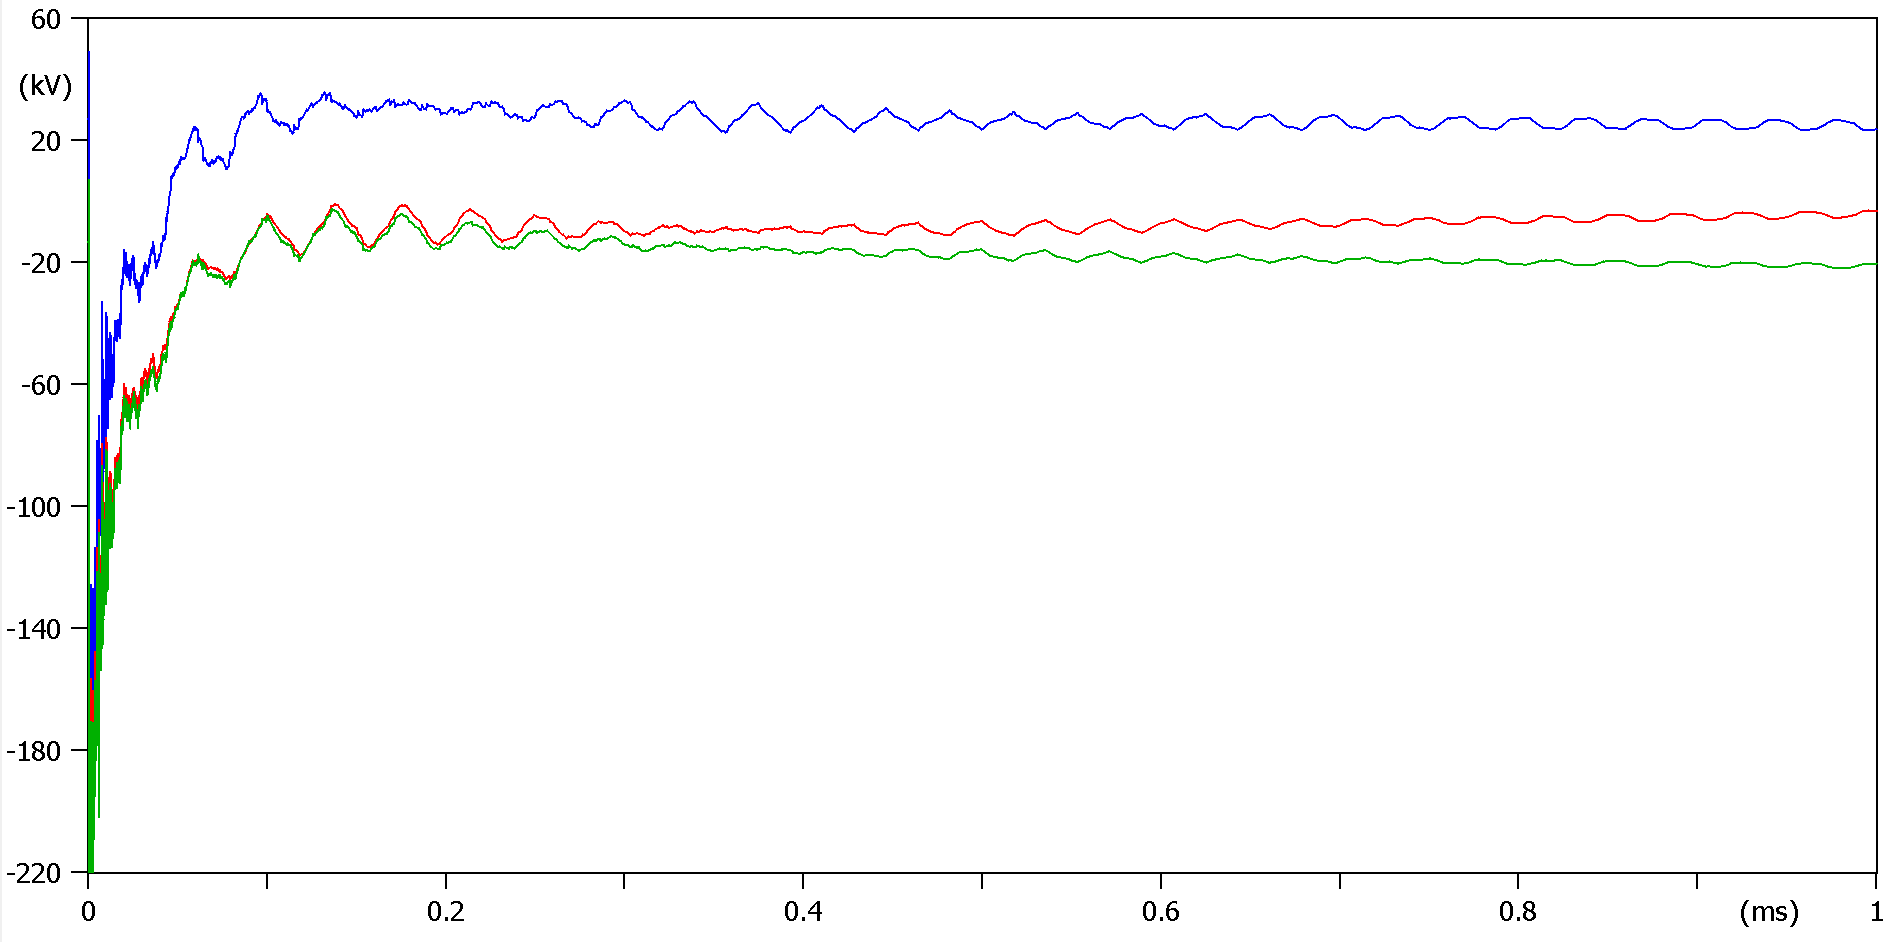
\includegraphics[width=\linewidth]{Figs/Resultados/40m_2.png}
        \caption{Detalle de la respuesta transitoria inicial para el contrapeso horizontal de 40 m.}
        \label{fig:contrapeso40_res2}
    \end{subfigure}

    \caption{Resultados obtenidos para la simulación del desempeño frente a descargas atmosféricas considerando un contrapeso horizontal de 40 m.}
    \label{fig:contrapeso40_resultados}
\end{figure}


\subsubsection{Contrapeso horizontal de 30 m}

Se evaluó una segunda alternativa consistente en un contrapeso horizontal de:

\begin{equation*}
l=30\ \mathrm{m}
\end{equation*}

Se obtuvo los parámetros distribuidos resumidos en la Tabla~\ref{tab:contrapeso30_parametros}.

\begin{table}[H]
\centering
\caption{Parámetros distribuidos obtenidos para el contrapeso horizontal de 30 m.}
\label{tab:contrapeso30_parametros}
\renewcommand{\arraystretch}{1.2}
\begin{tabular}{cccc}
\toprule
$R_i$ ($\Omega$) & $L_i$ (H) & $C_i$ (F) \\
\midrule
404.8944 &
$2.7257\times10^{-6}$ &
$7.5820\times10^{-10}$ \\
\bottomrule
\end{tabular}
\end{table}

La Figura~\ref{fig:contrapeso30_general} presenta la respuesta temporal de las tensiones desarrolladas sobre las fases durante la simulación, mientras que la Figura~\ref{fig:contrapeso30_zoom} muestra un acercamiento de los primeros instantes posteriores al impacto de la descarga atmosférica.

\begin{figure}[H]
    \centering

    \begin{subfigure}[t]{0.48\textwidth}
        \centering
        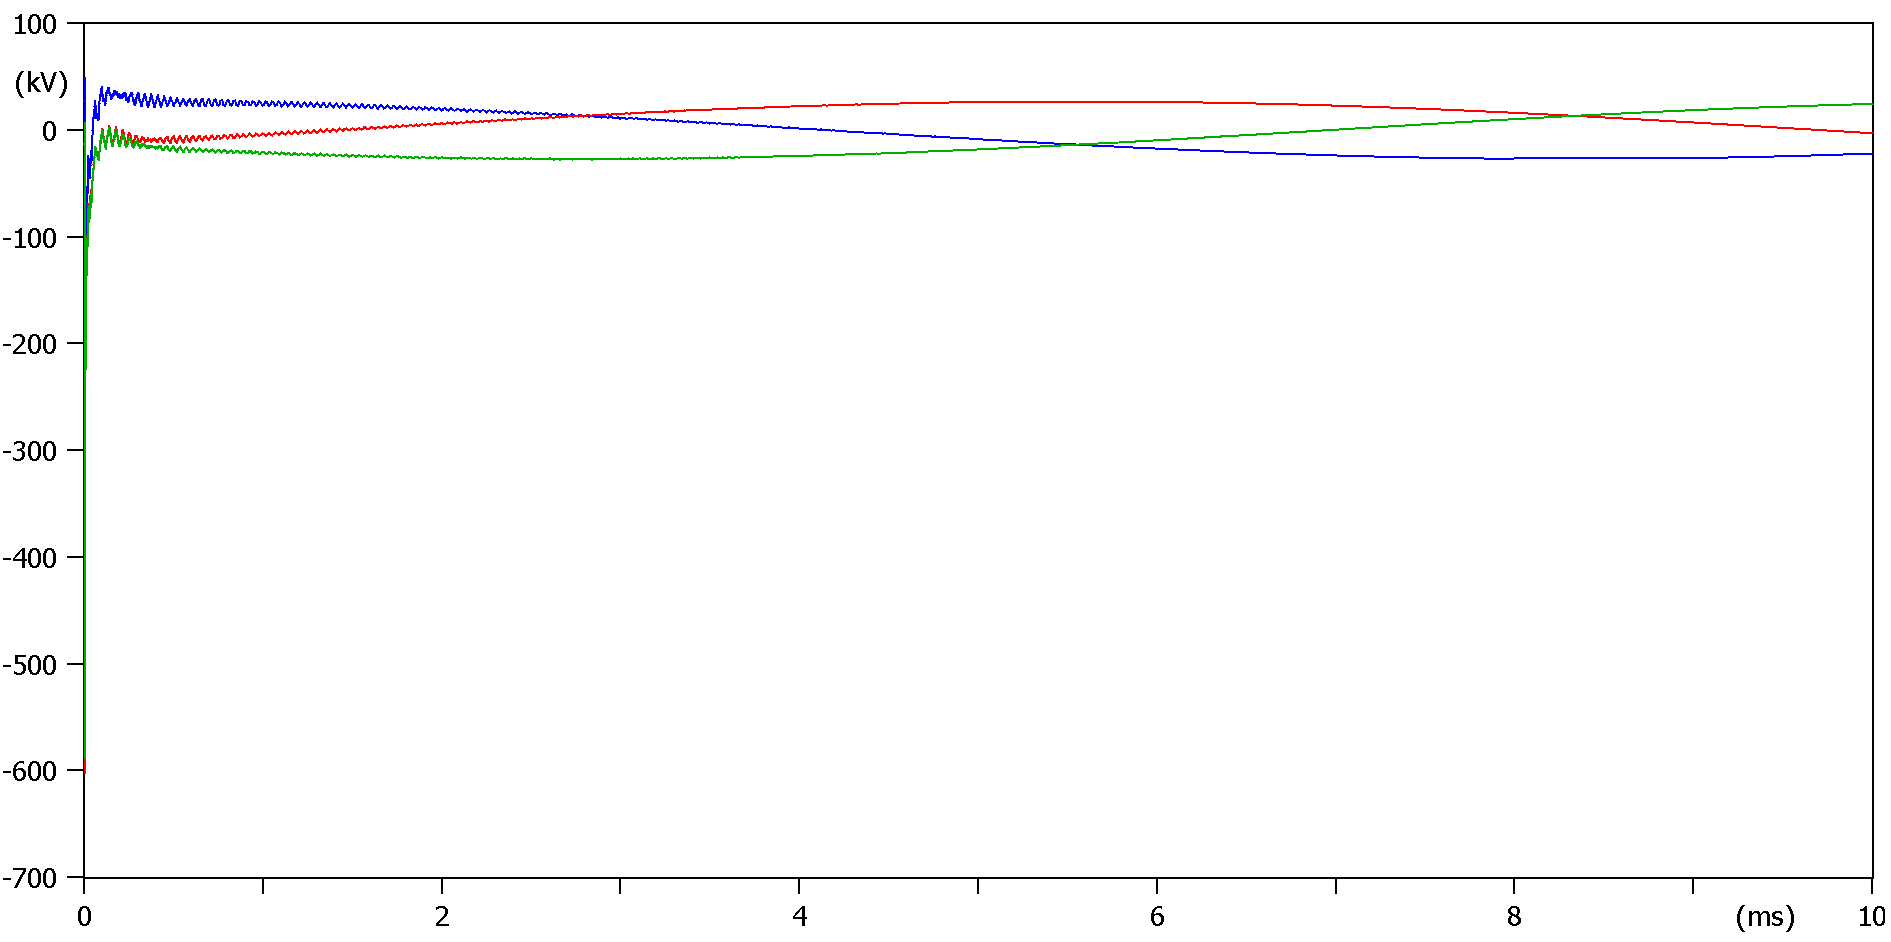
\includegraphics[width=\linewidth]{Figs/Resultados/30m_1.png}
        \caption{Respuesta temporal de las tensiones de fase para el contrapeso horizontal de 30 m.}
        \label{fig:contrapeso30_general}
    \end{subfigure}
    \hfill
    \begin{subfigure}[t]{0.48\textwidth}
        \centering
        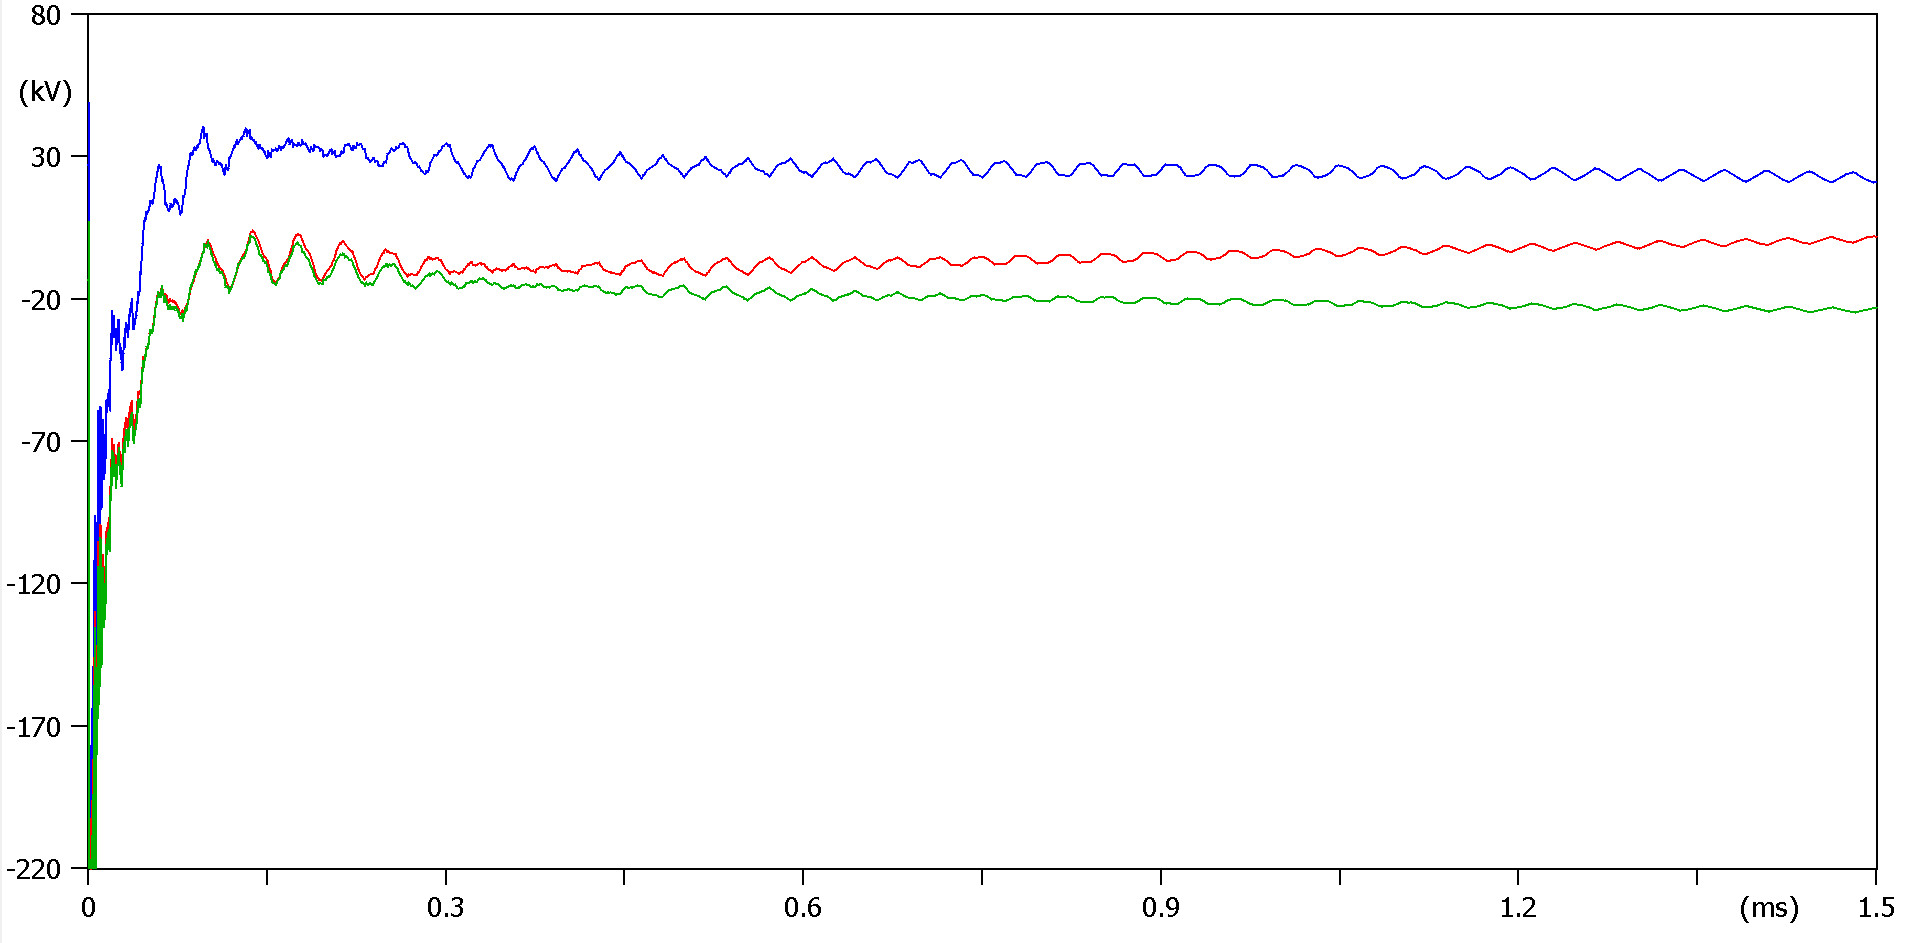
\includegraphics[width=\linewidth]{Figs/Resultados/30m_2.png}
        \caption{Detalle de la respuesta transitoria inicial para el contrapeso horizontal de 30 m.}
        \label{fig:contrapeso30_zoom}
    \end{subfigure}

    \caption{Resultados obtenidos para la simulación del desempeño frente a descargas atmosféricas considerando un contrapeso horizontal de 30 m.}
    \label{fig:contrapeso30_resultados}
\end{figure}

Al comparar los resultados con la configuración de 40 m, se observa un incremento moderado de las oscilaciones transitorias y de las sobretensiones desarrolladas sobre las fases durante los primeros instantes de la simulación. Sin embargo, las tensiones permanecen dentro de los límites de soportabilidad establecidos por el modelo Volt-Time, por lo que no se evidencia la ocurrencia de fenómenos de \textit{Backflashover}.

Los resultados obtenidos indican que la reducción de la longitud del contrapeso hasta 30 m no compromete el desempeño atmosférico de la estructura, manteniendo una capacidad adecuada de disipación de la corriente impulsiva hacia el terreno.

\subsubsection{Contrapeso horizontal de 20 m}

Continuando con el proceso de optimización, se evaluó una tercera configuración consistente en un contrapeso horizontal de:

\begin{equation*}
l=20\ \mathrm{m}
\end{equation*}

manteniendo las mismas condiciones de simulación utilizadas en las configuraciones anteriores. Los parámetros distribuidos obtenidos para esta longitud se resumen en la Tabla~\ref{tab:contrapeso20_parametros}.

\begin{table}[H]
\centering
\caption{Parámetros distribuidos obtenidos para el contrapeso horizontal de 20 m.}
\label{tab:contrapeso20_parametros}
\renewcommand{\arraystretch}{1.2}
\begin{tabular}{ccc}
\toprule
$R_i$ ($\Omega$) & $L_i$ (H) & $C_i$ (F) \\
\midrule
580.2383 &
$1.7361\times10^{-6}$ &
$4.8291\times10^{-10}$ \\
\bottomrule
\end{tabular}
\end{table}

La Figura~\ref{fig:contrapeso20} presenta la respuesta temporal obtenida para esta configuración, incluyendo tanto la evolución completa de las tensiones de fase como una ampliación de los primeros instantes posteriores al impacto del rayo.

\begin{figure}[H]
\centering

\begin{subfigure}[b]{0.48\textwidth}
    \centering
    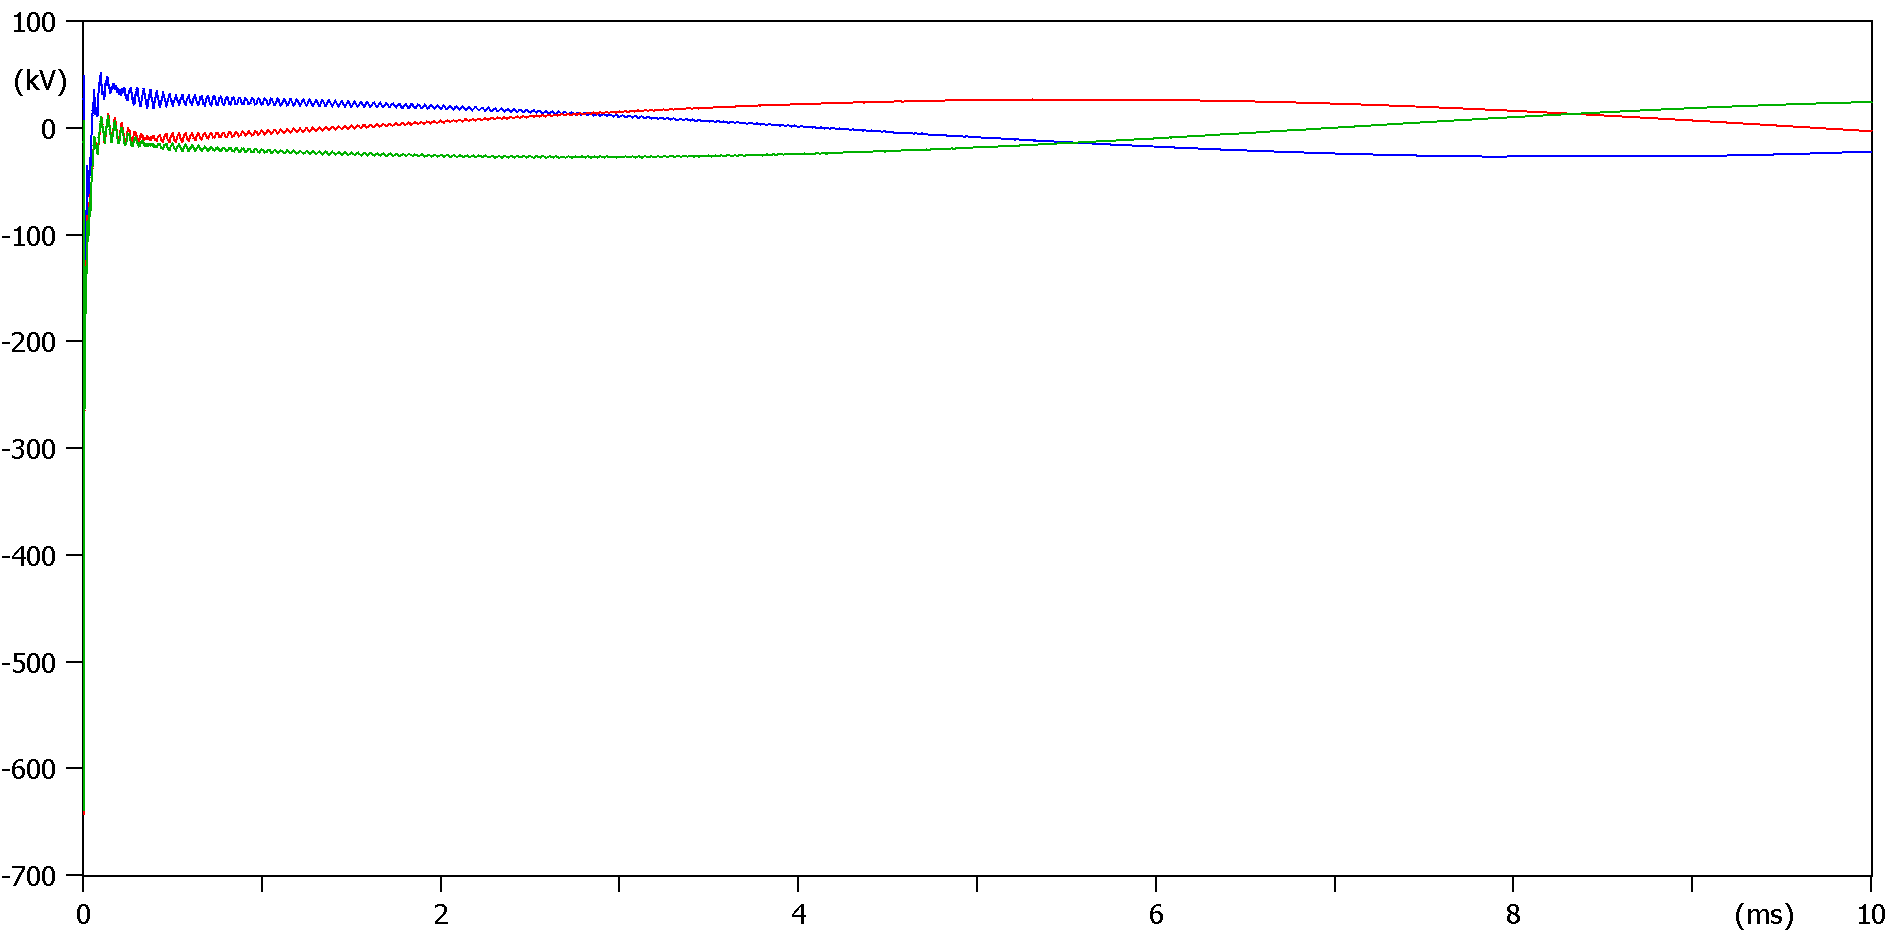
\includegraphics[width=\textwidth]{Figs/Resultados/20m_1.png}
    \caption{Respuesta temporal de las tensiones de fase para el contrapeso horizontal de 20 m.}
    \label{fig:contrapeso20_general}
\end{subfigure}
\hfill
\begin{subfigure}[b]{0.48\textwidth}
    \centering
    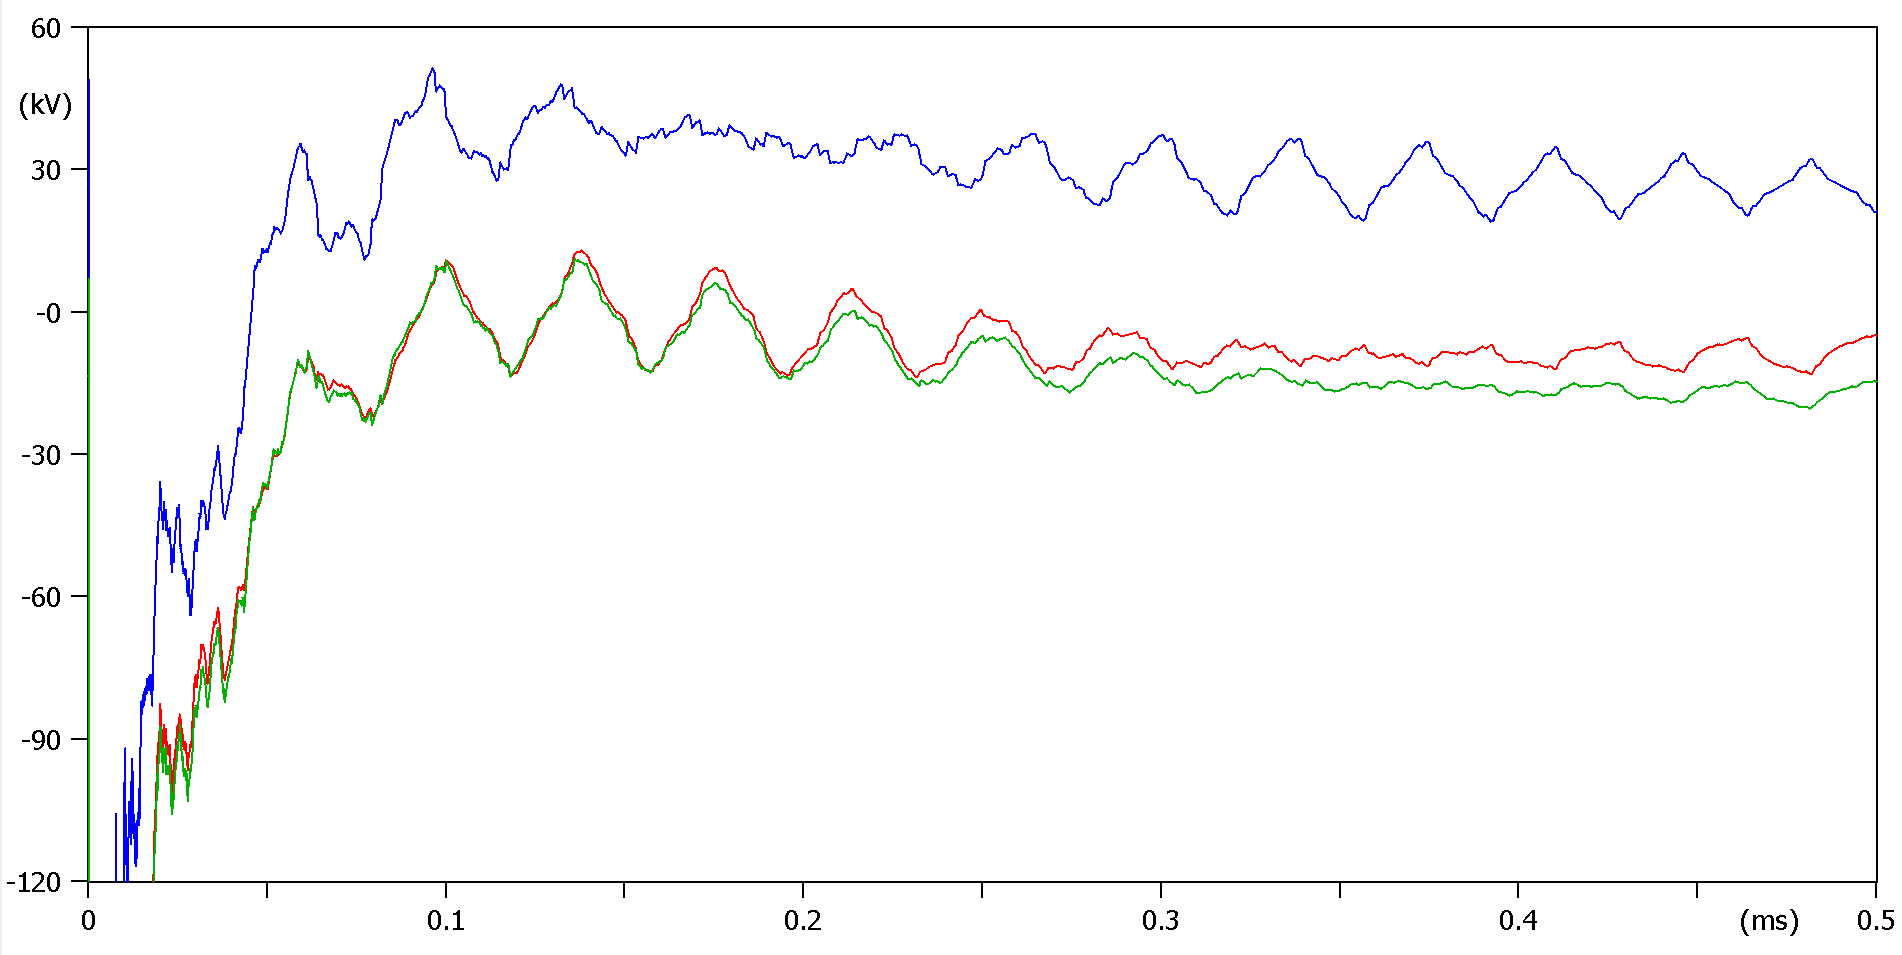
\includegraphics[width=\textwidth]{Figs/Resultados/20m_2.png}
    \caption{Detalle de la respuesta transitoria inicial para el contrapeso horizontal de 20 m.}
    \label{fig:contrapeso20_zoom}
\end{subfigure}

\caption{Resultados obtenidos para la simulación del desempeño frente a descargas atmosféricas considerando un contrapeso horizontal de 20 m.}
\label{fig:contrapeso20}

\end{figure}

Al igual que en los casos de 40 m y 30 m, no se observó la activación del modelo Volt-Time ni la ocurrencia de fenómenos de \textit{Backflashover}. Aunque la reducción de la longitud del contrapeso incrementó la resistencia distribuida equivalente del sistema de puesta a tierra, las sobretensiones desarrolladas sobre las cadenas de aislamiento permanecieron dentro de los límites de soportabilidad del aislamiento.

Los resultados obtenidos indican que una longitud de 20 m continúa proporcionando una trayectoria efectiva para la disipación de la corriente impulsiva, manteniendo un desempeño atmosférico satisfactorio y reduciendo simultáneamente la cantidad de conductor requerido respecto a las alternativas previamente evaluadas.

\subsubsection{Contrapeso horizontal de 10 m}

Finalmente, se evaluó una configuración con un contrapeso horizontal de:

\begin{equation*}
l=10\ \mathrm{m}
\end{equation*}

manteniendo los mismos criterios de modelado y condiciones de simulación empleados en los casos anteriores. Los parámetros distribuidos obtenidos para esta longitud se resumen en la Tabla~\ref{tab:contrapeso10_parametros}.

\begin{table}[H]
\centering
\caption{Parámetros distribuidos obtenidos para el contrapeso horizontal de 10 m.}
\label{tab:contrapeso10_parametros}
\renewcommand{\arraystretch}{1.2}
\begin{tabular}{ccc}
\toprule
$R_i$ ($\Omega$) & $L_i$ (H) & $C_i$ (F) \\
\midrule
1067.8096 &
$7.9872\times10^{-7}$ &
$2.2217\times10^{-10}$ \\
\bottomrule
\end{tabular}
\end{table}

La Figura~\ref{fig:contrapeso10} presenta la respuesta temporal obtenida para esta configuración.

\begin{figure}[H]
\centering

\begin{subfigure}[b]{0.48\textwidth}
    \centering
    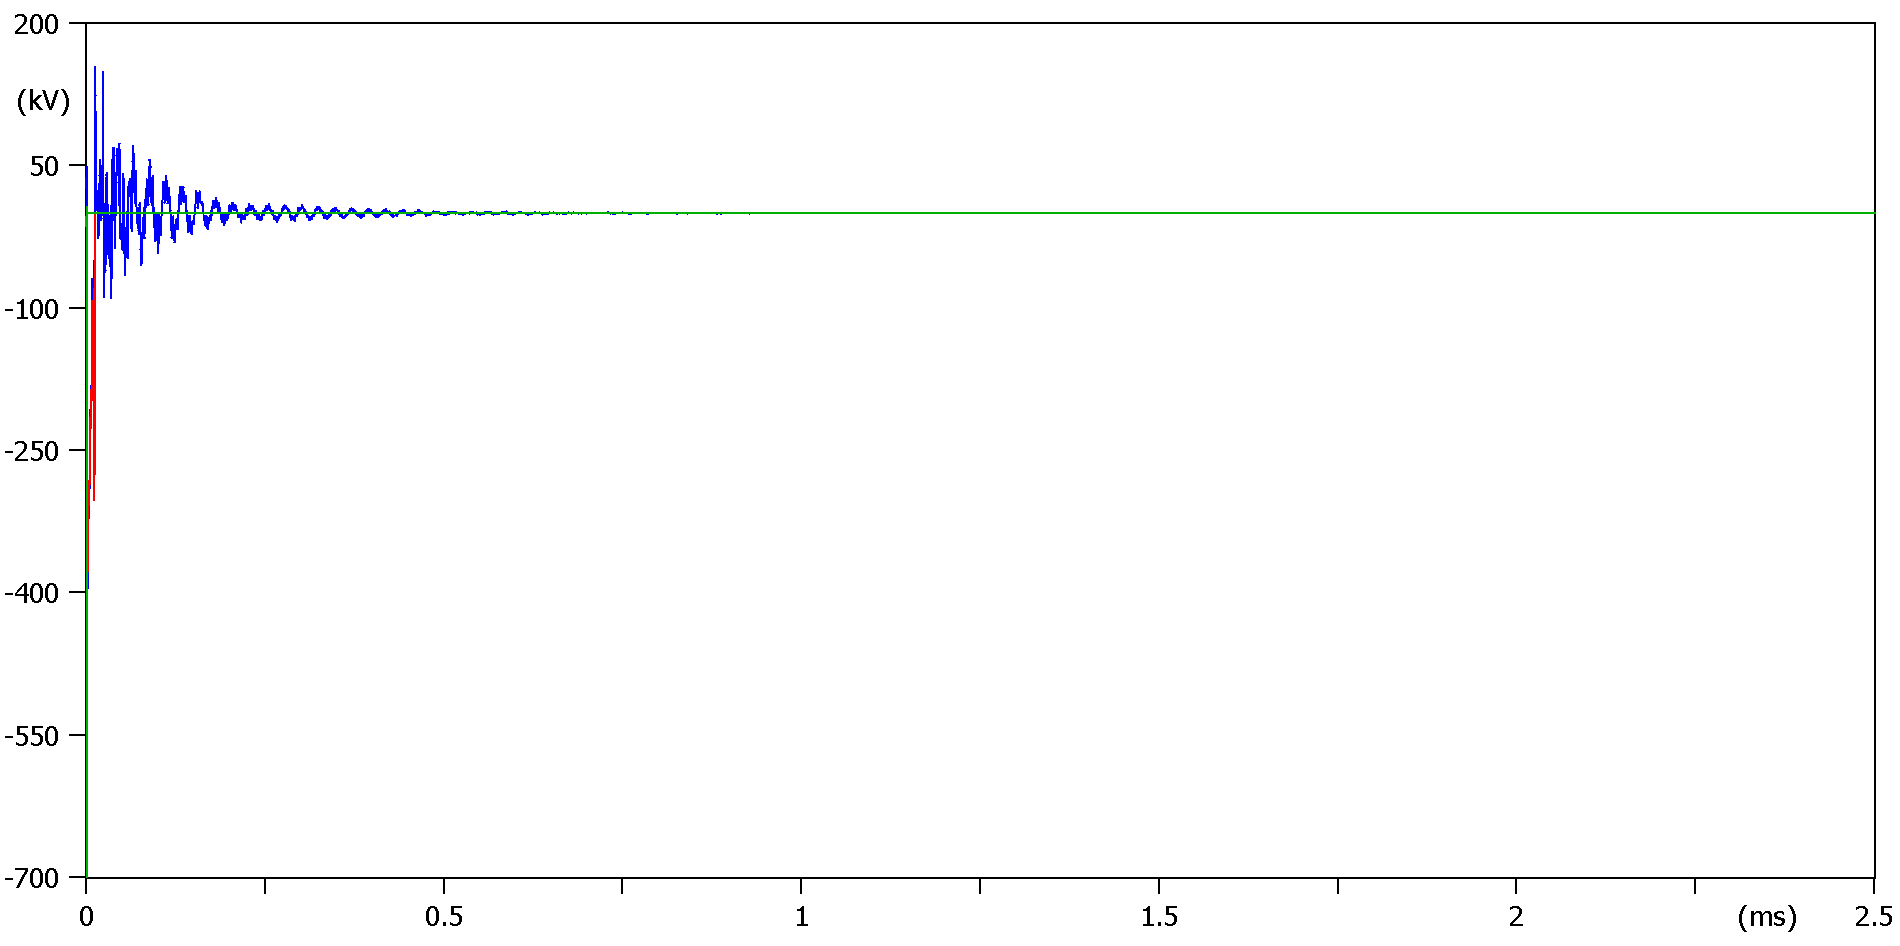
\includegraphics[width=\textwidth]{Figs/Resultados/10m_1.png}
    \caption{Respuesta temporal de las tensiones de fase para el contrapeso horizontal de 10 m.}
    \label{fig:contrapeso10_general}
\end{subfigure}
\hfill
\begin{subfigure}[b]{0.48\textwidth}
    \centering
    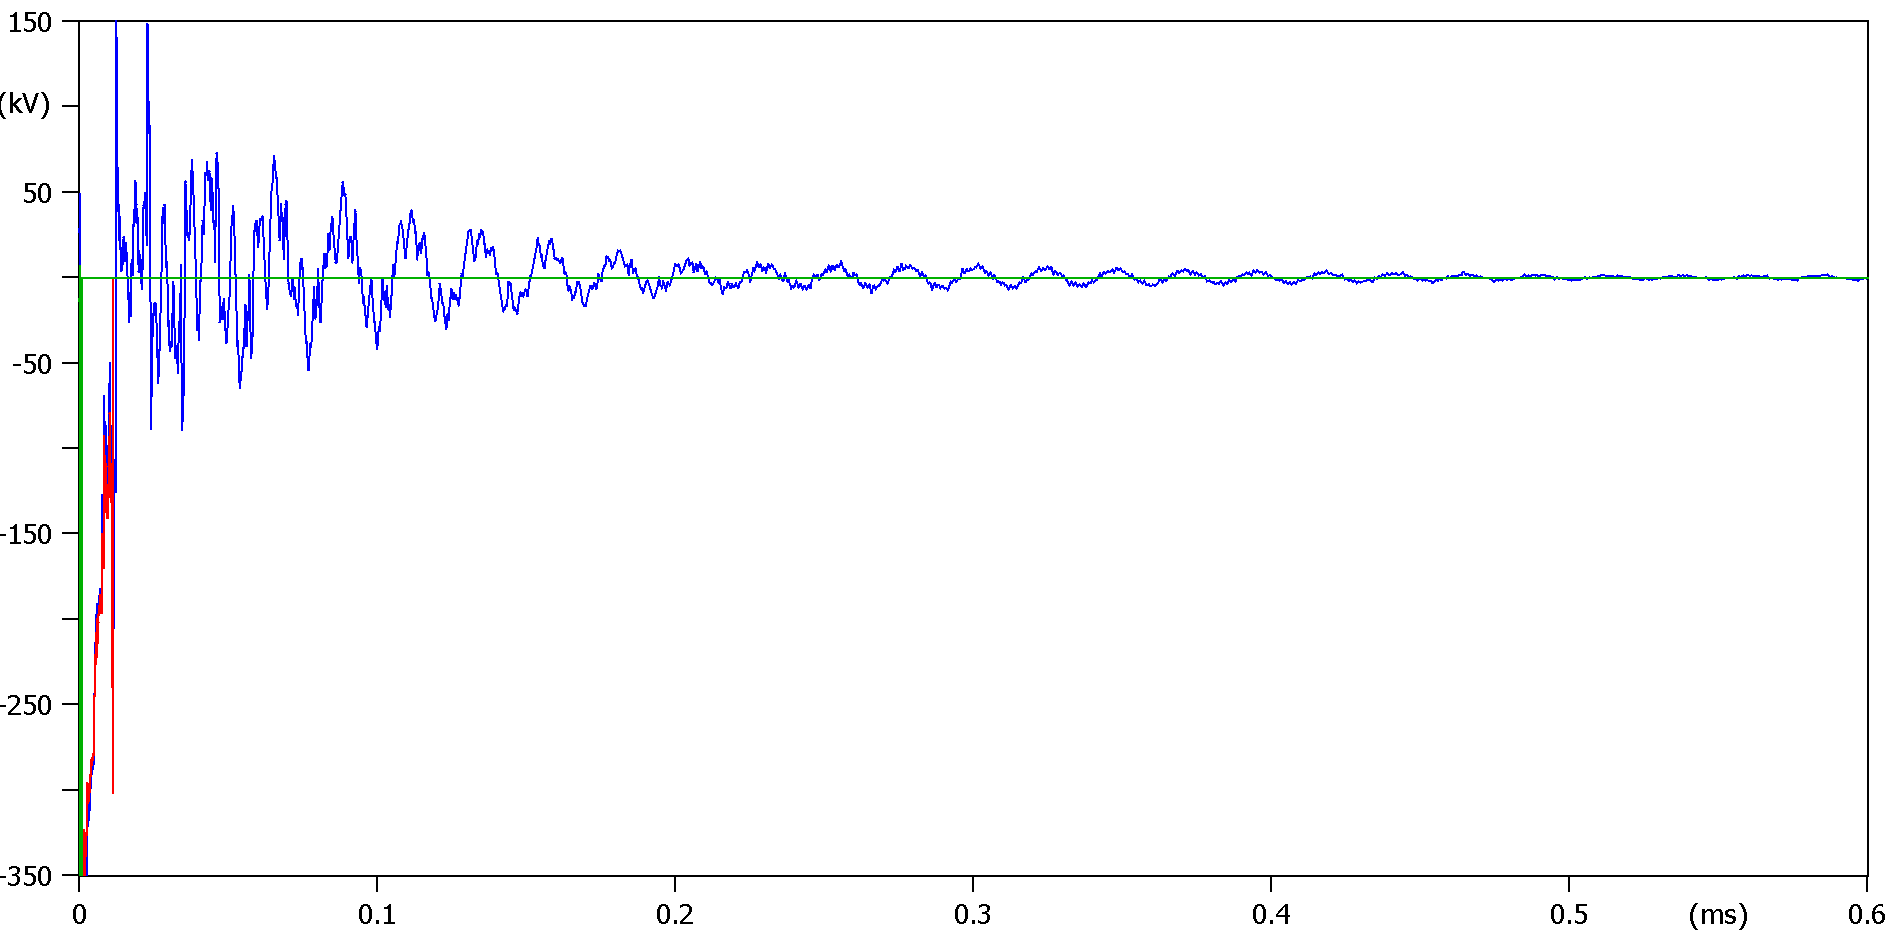
\includegraphics[width=\textwidth]{Figs/Resultados/10m_2.png}
    \caption{Detalle de la respuesta transitoria inicial para el contrapeso horizontal de 10 m.}
    \label{fig:contrapeso10_zoom}
\end{subfigure}

\caption{Resultados obtenidos para la simulación del desempeño frente a descargas atmosféricas considerando un contrapeso horizontal de 10 m.}
\label{fig:contrapeso10}

\end{figure}

A diferencia de las configuraciones previamente evaluadas, la reducción de la longitud del contrapeso a 10 m produjo un incremento significativo de la impedancia equivalente del sistema de puesta a tierra, reflejado en mayores amplitudes de sobretensión y una respuesta oscilatoria más severa durante los primeros instantes posteriores al impacto del rayo.

Los resultados obtenidos evidencian la ocurrencia de un fenómeno de \textit{Backflashover} (\textit{BFO}), indicando que la capacidad de disipación de corriente proporcionada por esta configuración resulta insuficiente para mantener la tensión sobre las cadenas de aislamiento dentro de la región de soportabilidad definida por el modelo Volt-Time.

Por consiguiente, la longitud de 10 m fue descartada como alternativa de diseño, estableciéndose que la longitud mínima capaz de evitar la ocurrencia de fenómenos de \textit{Backflashover} corresponde a 20 m.


\subsection{Diseño final seleccionado}

Las simulaciones realizadas para las configuraciones de 40 m, 30 m, 20 m y 10 m permitieron identificar que la longitud mínima capaz de evitar la ocurrencia de fenómenos de \textit{Backflashover} correspondía a 20 m. Por esta razón, dicha configuración fue seleccionada inicialmente para continuar con la evaluación del sistema de puesta a tierra.

La Tabla~\ref{tab:resumen_contrapesos} resume los resultados obtenidos durante el proceso de optimización.

\begin{table}[H]
\centering
\caption{Resumen de configuraciones evaluadas para los contrapesos horizontales.}
\label{tab:resumen_contrapesos}
\renewcommand{\arraystretch}{1.2}
\begin{tabular}{ccc}
\toprule
Longitud (m) & BFO & Estado \\
\midrule
40 & No & Aceptable \\
30 & No & Aceptable \\
20 & No & Seleccionada preliminarmente \\
10 & Sí & Descartada \\
\bottomrule
\end{tabular}
\end{table}

Una vez definida la longitud preliminar del contrapeso, se procedió a calcular la resistencia equivalente del sistema de puesta a tierra con el fin de verificar su desempeño frente a los criterios utilizados posteriormente en la evaluación estadística mediante IEEE Flash.

Para el modelado del sistema de puesta a tierra del apoyo tipo "Tormenta" se consideró una configuración compuesta por la resistencia equivalente de la estructura, los contrapesos horizontales y el electrodo vertical, todos conectados eléctricamente en paralelo. La resistencia total se determinó mediante:

\begin{equation}
\frac{1}{R_{total}}
=
\frac{1}{Z_{eq\_A173}}
+
\frac{n_h}{R_{horiz}}
+
\frac{n_v}{R_{vert}}
\label{eq:Rtotal}
\end{equation}

donde:

\begin{itemize}
    \item $Z_{eq\_A173}=87.2586\ \Omega$ corresponde a la resistencia equivalente del apoyo A173.
    \item $R_{horiz}=29.0119\ \Omega$ corresponde a la resistencia de cada contrapeso horizontal.
    \item $R_{vert}=182.7121\ \Omega$ corresponde a la resistencia del electrodo vertical.
    \item $n_h$ es el número de contrapesos horizontales.
    \item $n_v$ es el número de electrodos verticales.
\end{itemize}

Inicialmente se evaluó la configuración conformada por un único contrapeso horizontal de 20 m ($n_h=1$) y un electrodo vertical ($n_v=1$). Sustituyendo en la Ecuación~\eqref{eq:Rtotal}:

\begin{equation*}
\frac{1}{R_{total}}
=
\frac{1}{87.2586}
+
\frac{1}{29.0119}
+
\frac{1}{182.7121}
\end{equation*}

\begin{equation*}
\frac{1}{R_{total}}
=
0.01146
+
0.03447
+
0.00547
=
0.05140
\end{equation*}

obteniéndose:

\begin{equation}
R_{total}=19.46\ \Omega
\end{equation}

Si bien esta configuración evitaba la ocurrencia de fenómenos de \textit{Backflashover} en las simulaciones transitorias realizadas en ATPDraw, el valor obtenido para la resistencia equivalente aún se consideró elevado para los criterios de desempeño atmosférico establecidos en IEEE Flash.

Por esta razón se evaluó una configuración mejorada incorporando un segundo contrapeso horizontal de 20 m conectado en paralelo al sistema existente. Las Figuras~\ref{fig:diseno_final_general} y \ref{fig:diseno_final_zoom} presentan la respuesta obtenida para esta configuración.

\begin{figure}[H]
\centering

\begin{subfigure}[b]{0.48\textwidth}
    \centering
    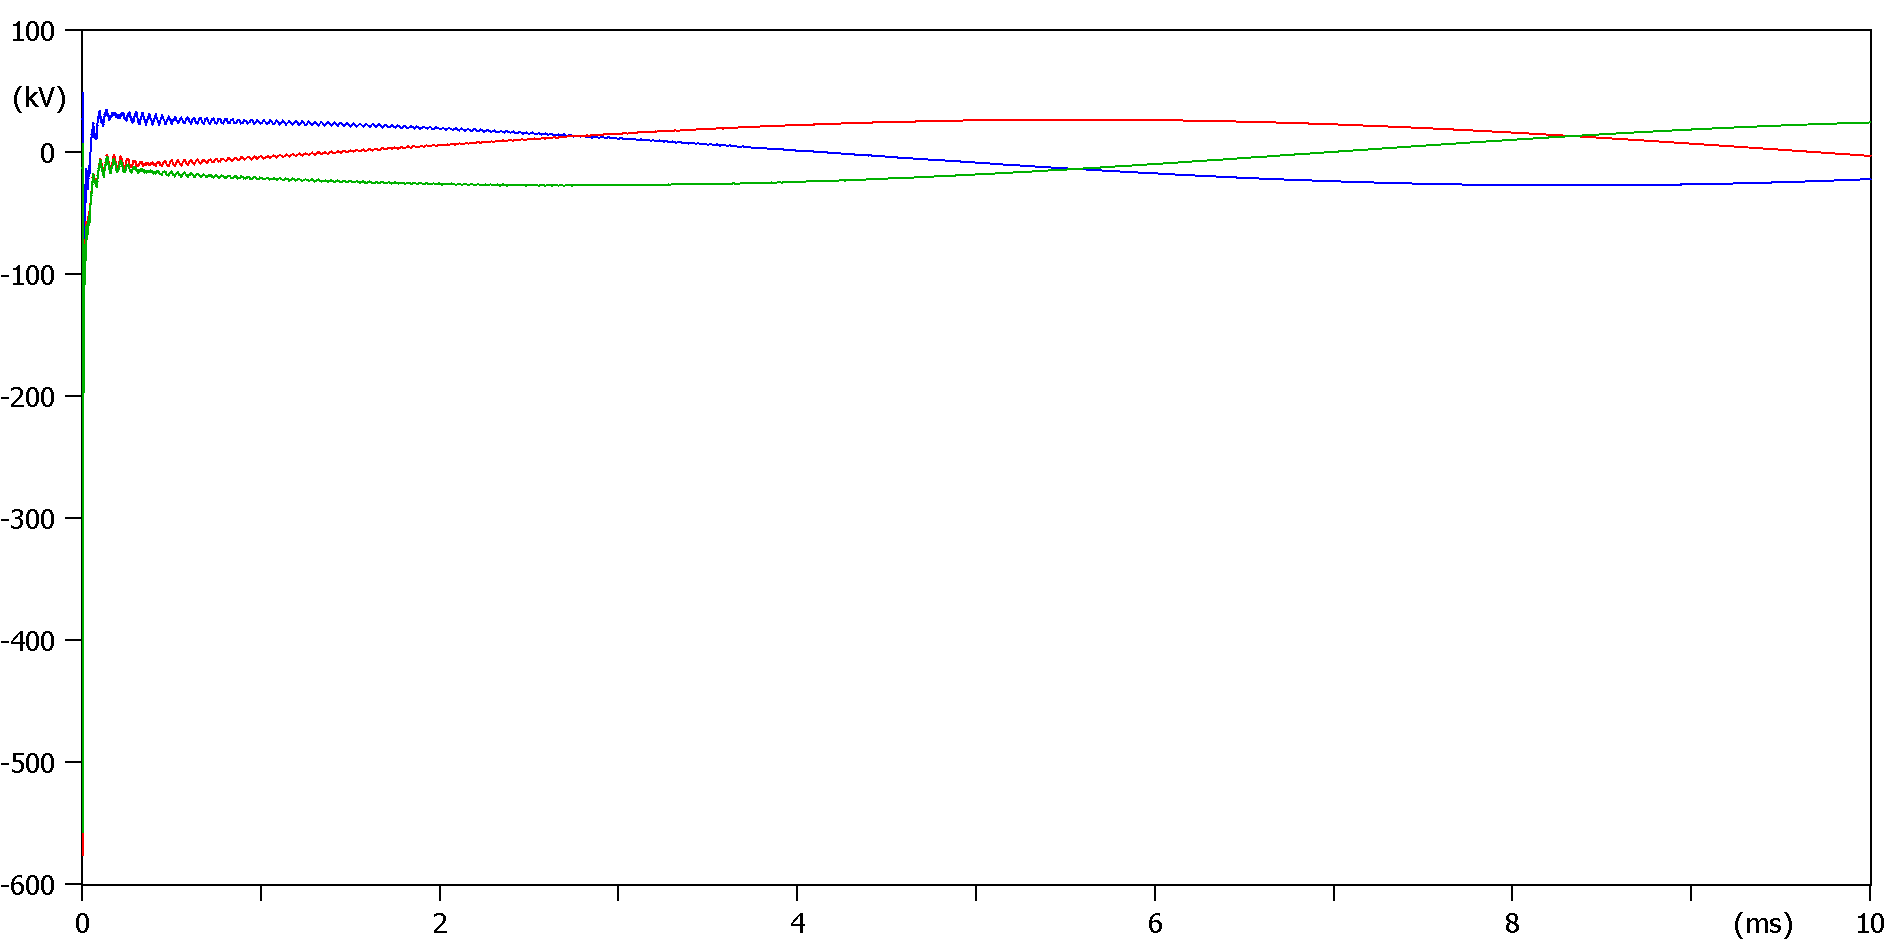
\includegraphics[width=\textwidth]{Figs/Resultados/20mx2_1.png}
    \caption{Respuesta temporal de las tensiones de fase para 2 contrapesos horizontales de 20 m.}
    \label{fig:diseno_final_general}
\end{subfigure}
\hfill
\begin{subfigure}[b]{0.48\textwidth}
    \centering
    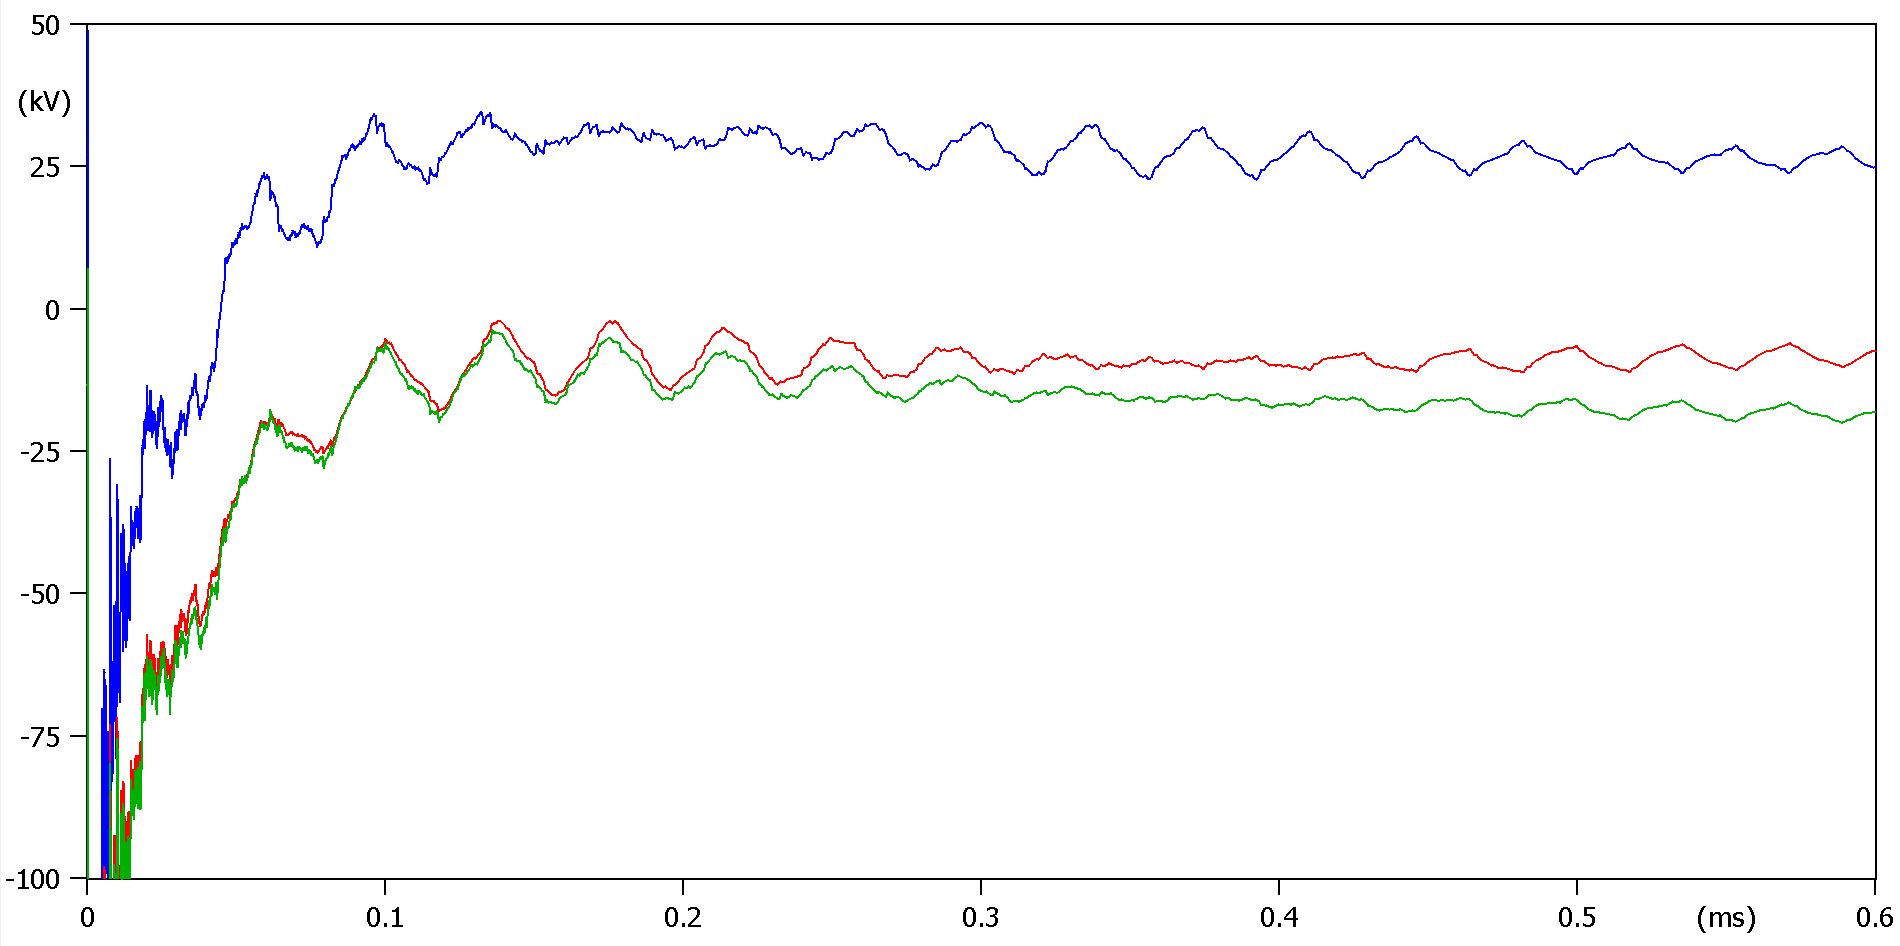
\includegraphics[width=\textwidth]{Figs/Resultados/20mx2_2.png}
    \caption{Detalle de la respuesta transitoria inicial para 2 contrapesos horizontales de 20 m.}
    \label{fig:diseno_final_zoom}
\end{subfigure}

\caption{Respuesta de las tensiones de fase para la configuración final del sistema de puesta a tierra.}
\label{fig:diseno_final}

\end{figure}

Para esta configuración final se consideró:

\begin{equation}
n_h=2
\end{equation}

\begin{equation}
n_v=1
\end{equation}

por lo que la resistencia equivalente se calculó como:

\begin{equation*}
\frac{1}{R_{total}}
=
\frac{1}{87.2586}
+
\frac{2}{29.0119}
+
\frac{1}{182.7121}
\end{equation*}

\begin{equation*}
\frac{1}{R_{total}}
=
0.01146
+
0.06894
+
0.00547
=
0.08587
\end{equation*}

obteniéndose finalmente:

\begin{equation}
R_{total}=11.65\ \Omega
\end{equation}

La incorporación del segundo contrapeso permitió reducir significativamente la resistencia equivalente del sistema de puesta a tierra, manteniendo simultáneamente la ausencia de fenómenos de \textit{Backflashover} observada en las simulaciones transitorias. En consecuencia, la configuración definitiva quedó conformada por dos contrapesos horizontales de 20 m y un electrodo vertical de 2.4 m, siendo esta la alternativa seleccionada para la evaluación estadística posterior mediante IEEE Flash.



\section{Evaluación del Desempeño Mediante IEEE Flash}

El comportamiento frente a descargas atmosféricas de la línea de subtransmisión de 33~kV se evaluó mediante el software especializado IEEE Flash (Version 2.04), implementando los modelos analíticos normalizados por la IEEE para el cálculo de tasas de salida por flameo inverso (\textit{backflashover}) y fallas de apantallamiento (\textit{shielding failures}). Para este análisis se parametrizó el nodo crítico A173, el cual cuenta geométricamente con un apoyo estructural real tipo ``Tormenta'' (configuración de tres postes en línea), el cual debió ser aproximado mediante el modelo en H debido a las opciones de modelado disponibles en la interfaz del programa.

\subsection{Parámetros de entrada y memorias de cálculo}

Los parámetros geométricos, eléctricos y ambientales se consolidaron a partir de la tabla con los parámetros suministrados. A continuación se detallan los criterios de cálculo y la procedencia de los datos ingresados al programa para el modelado del Nodo A173:

\begin{itemize}
	\item \textbf{Densidad de Descargas a Tierra ($N_g$):} Se configuró un valor crítico de $78.77\text{ rayos/km}^2/\text{año}$, consistente con la alta actividad de rayos registrada para la zona de estudio, con un vano (\textit{Span}) fijado en $23.8\text{ m}$.
	\item \textbf{Conductores de Fase:} Corresponden al calibre 2/0~ACSR~AW. El diámetro exterior se obtuvo a partir del radio externo de la capa de aluminio especificado en la tabla ($r_{ext} = 0.5675\text{ cm}$):
	\begin{equation}
		D_{cond} = 2 \times 0.5675\text{ cm} = 1.135\text{ cm} = 11.35\text{ mm}
	\end{equation}
	La tensión de operación fase-tierra máxima ingresada en el programa se determinó mediante la relación entre tensiones fase-fase y fase-tierra:
	\begin{equation}
		V_{ln} = \frac{33\text{ kV}}{\sqrt{3}} \approx 19.05\text{ kV}
	\end{equation}
	La disposición espacial se configuró en una geometría horizontal simétrica con coordenadas $X = \{-2.5, 0, 2.5\}\text{ m}$, una altura de fijación en el apoyo de $Y = 9.8\text{ m}$.
	La flecha o pandeo (\textit{Sag}) de los conductores de fase se determinó usando los datos de la altura y la altura media de las fases:
	\begin{equation}
		Sag = 9.8\text{ m} - 9\text{ m} = 0.8\text{ m}
	\end{equation}
	\item \textbf{Distancia de Aislamiento (\textit{Strike Distance}, SI):} A partir de la longitud efectiva de la cadena de aisladores (4 discos de porcelana café de $10.7''$), equivalente a $58.40\text{ cm}$, se parametrizó un valor de $SI = 0.584\text{ m}$.
	\item \textbf{Cable de Guarda:} Se especificó un cable de acero/aluminio de $1/4''$ con un diámetro nominal de $6.35\text{ mm}$. El cable se posicionó centralmente a una altura $Y = 12.7\text{ m}$ para garantizar el ángulo de protección requerido. La flecha del cable de guarda se determinó mediante la altura y la altura media del cable de guarda:
	\begin{equation}
		Sag = 12.7\text{ m} - 12.07\text{ m} = 0.63\text{ m}
	\end{equation}
	\item \textbf{Modelado de Estructura y Puesta a Tierra:} La estructura real en el Nodo A173 corresponde a un apoyo tipo ``Tormenta''. Al no disponer el software de un modelo nativo para este tipo de apoyo, se seleccionó el modelo \textit{H-Frame} como la aproximación disponible más adecuada para imitar los caminos de descarga paralelos. La altura expuesta es de $10\text{ m}$, la separación entre postes externos (\textit{Lead Separation}) se fijó en $1.8\text{ m}$ y el diámetro equivalente se determinó mediante el radio en la base y diámetro en la cima del poste:
	\begin{equation}
		D_{eq} = \frac{2 \times 0.26\text{ m} + 0.15\text{ m}}{2} = 0.335\text{ m}
	\end{equation}
	\item \textbf{Resistencia a Pie de Torre ($R_{total}$):} Una vez seleccionada la configuración definitiva del sistema de puesta a tierra, compuesta por dos contrapesos horizontales de 20 m y un electrodo vertical de 2.4 m, se determinó la resistencia equivalente a pie de torre mediante la asociación en paralelo de las impedancias correspondientes al apoyo, los contrapesos horizontales y el electrodo vertical.

    Considerando los valores obtenidos previamente para cada uno de estos elementos, se obtuvo una resistencia equivalente de:
    
    \begin{equation}
    R_{total}=11.6454\ \Omega
    \end{equation}
    
    Este valor fue empleado como parámetro de entrada en la sección \textit{Footing Resistances} del software IEEE Flash para la evaluación estadística del desempeño atmosférico del tramo estudiado.
\end{itemize}

El resumen total de los datos de entrada se detalla en el Cuadro~\ref{tab:parametros_flash_A173}.

\begin{table}[H]
	\centering
	\caption{Parámetros de entrada consolidados para la simulación del Nodo A173.}
	\label{tab:parametros_flash_A173}
	\begin{tabular}{lc}
		\toprule
		\textbf{Parámetro de Entrada} & \textbf{Valor Registrado} \\
		\midrule
		Modelo Equivalente de Estructura & 2 - H Frame \\
		Tipo de Estructura Real & Tormenta (Pórtico Triple) \\
		Altura de la Estructura $H$ (m) & 10.0 \\
		Diámetro Equivalente del Poste (m) & 0.335 \\
		Separación de Postes en Modelo $d$ (m) & 1.8 \\
		Densidad de Rayos $N_g$ ($\text{rayos/km}^2/\text{año}$) & 78.77 \\
		Longitud del Vano (m) & 23.8 \\
		Diámetro del Conductor de Fase (mm) & 11.35 \\
		Flecha del Conductor de Fase (\textit{Sag}) (m) & 0.8 \\
		Voltaje de Operación Fase-Tierra (kV) & 19.05 \\
		Distancia de Arqueo / Aislamiento $SI$ (m) & 0.584 \\
		Diámetro del Cable de Guarda (mm) & 6.35 \\
		Flecha del Cable de Guarda (\textit{Sag}) (m) & 0.63 \\
		Resistencia a Pie de Torre Calculada $R_{total}$ ($\Omega$) & 11.6454 \\
		\bottomrule
	\end{tabular}
\end{table}

\subsection{Resultados obtenidos}

Tras ejecutar la simulación del escenario del Nodo A173, el software determinó las corrientes críticas necesarias para causar la disrupción dieléctrica del aislamiento por cada fase, así como las tasas estadísticas de salidas por cada 100~km de línea al año. Los resultados numéricos se exponen detalladamente en el Cuadro~\ref{tab:resultados_flash_A173}.

\begin{table}[H]
	\centering
	\caption{Resultados de tasas de falla y corrientes críticas para el Nodo A173.}
	\label{tab:resultados_flash_A173}
	\begin{tabular}{lc}
		\toprule
		\textbf{Índice de desempeño} & \textbf{Valor Calculado} \\
		\midrule
		\textbf{Corrientes críticas de flameo ($I_{crit}$)} & \\
		~~Fase izquierda / Conductor 1 (kA) & 43.89 \\
		~~Fase central / Conductor 2 (kA) & 45.59 \\
		~~Fase derecha / Conductor 3 (kA) & 43.94 \\
		\midrule
		\textbf{Corrientes críticas de apantallamiento} & \\
		~~Conductor 1 (kA) & 1.60 \\
		~~Conductor 3 (kA) & 6.16 \\
		\midrule
		\textbf{Tasas de salida ($\text{fallas/100 km/año}$)} & \\
		~~Tasa por flameo inverso (\textit{Backflash rate}) & 173.89 \\
		~~Tasa por falla de apantallamiento (\textit{Shielding failure rate}) & 0.62 \\
		\midrule
		\textbf{Tasa de salidas total} & \textbf{174.51} \\
		\bottomrule
	\end{tabular}
\end{table}

\subsection{Análisis de los índices de desempeño}

El análisis de los indicadores obtenidos para el Nodo A173 permite establecer las siguientes observaciones:

\begin{enumerate}
	\item \textbf{Predominio del fenómeno de Backflashover:} La tasa total de salidas calculada fue de \SI{174.51}{fallas/100.\km/a\tilde{n}o}, de las cuales \SI{173.89}{fallas/100.\km/a\tilde{n}o} corresponden a flameos inversos (\textit{Backflashover}). Esto evidencia que el principal mecanismo de falla continúa siendo la elevación transitoria del potencial de la estructura durante impactos directos de rayo sobre el cable de guarda o la torre. La elevada actividad atmosférica de la zona ($N_g=\SI{78.77}{rayos/km^2/a\tilde{n}o}$) incrementa significativamente la probabilidad de ocurrencia de este fenómeno.
	
	\item \textbf{Capacidad de soportabilidad del aislamiento:} Las corrientes críticas obtenidas fueron de \SI{43.89}{\kA}, \SI{45.59}{\kA} y \SI{43.94}{\kA} para las fases izquierda, central y derecha, respectivamente. Estos valores indican que el aislamiento es capaz de soportar descargas atmosféricas de magnitud moderada, mientras que impactos con corrientes superiores a aproximadamente \SI{44}{\kA} pueden provocar la disrupción dieléctrica y el consecuente flameo inverso.
	
	\item \textbf{Desempeño del sistema de blindaje:} La tasa de falla de apantallamiento obtenida fue de únicamente \SI{0.62}{fallas/100.\km/a\tilde{n}o}, valor considerablemente inferior a la tasa de Backflashover. Las corrientes críticas de blindaje calculadas fueron de \SI{1.60}{\kA} para el conductor 1 y \SI{6.16}{\kA} para el conductor 3, lo que confirma que la disposición geométrica del cable de guarda proporciona una protección adecuada frente a impactos directos sobre los conductores de fase.
	
	\item \textbf{Evaluación global del desempeño:} Aunque la configuración final de puesta a tierra logró una resistencia equivalente de \SI{11.6454}{\Omega}, la tasa total de salidas permanece elevada debido a las severas condiciones atmosféricas presentes en la zona de estudio. Esto indica que la optimización de la puesta a tierra mejora el comportamiento de la estructura, pero no resulta suficiente para eliminar completamente el riesgo de Backflashover.
\end{enumerate}

%---------------------------------------------


\section{Análisis de Resultados}

\subsection{Influencia de la longitud de los contrapesos}

La longitud de los contrapesos horizontales constituye uno de los parámetros más influyentes en el desempeño transitorio del sistema de puesta a tierra frente a descargas atmosféricas. En este caso, se evaluaron cuatro alternativas de diseño correspondientes a longitudes de 40 m, 30 m, 20 m y 10 m, manteniendo constantes las demás características geométricas y eléctricas del sistema.

A partir de las expresiones desarrolladas previamente para el modelo distribuido de los contrapesos, se obtuvo que al disminuir la longitud del conductor enterrado aumenta la resistencia serie equivalente y disminuyen los parámetros inductivos y capacitivos asociados. Como consecuencia, la capacidad del sistema para disipar la corriente impulsiva del rayo se reduce progresivamente, generando mayores elevaciones de potencial en la estructura.

Las simulaciones electromagnéticas realizadas en ATPDraw permitieron verificar este comportamiento. Para las configuraciones de 40 m, 30 m y 20 m se observó una adecuada disipación de la corriente de descarga, manteniéndose las tensiones desarrolladas sobre las cadenas de aisladores por debajo de los niveles críticos de ruptura definidos por el modelo \textit{Volt-Time}. En consecuencia, no se presentó la ocurrencia de fenómenos de \textit{Backflashover}.

Por el contrario, la configuración de 10 m presentó un comportamiento significativamente diferente. La reducción de la longitud del contrapeso produjo un incremento importante de la impedancia transitoria del sistema de puesta a tierra, elevando el potencial de la estructura durante la descarga atmosférica. Bajo estas condiciones, la tensión aplicada sobre el aislamiento superó la característica de soportabilidad \textit{Volt-Time}, provocando la operación del modelo de ruptura y la consecuente ocurrencia de un \textit{Backflashover}.

La Figura~\ref{fig:comparacion_contrapesos} resume la respuesta obtenida para las distintas longitudes evaluadas.

\begin{figure}[H]
\centering

\begin{subfigure}[b]{0.48\textwidth}
    \centering
    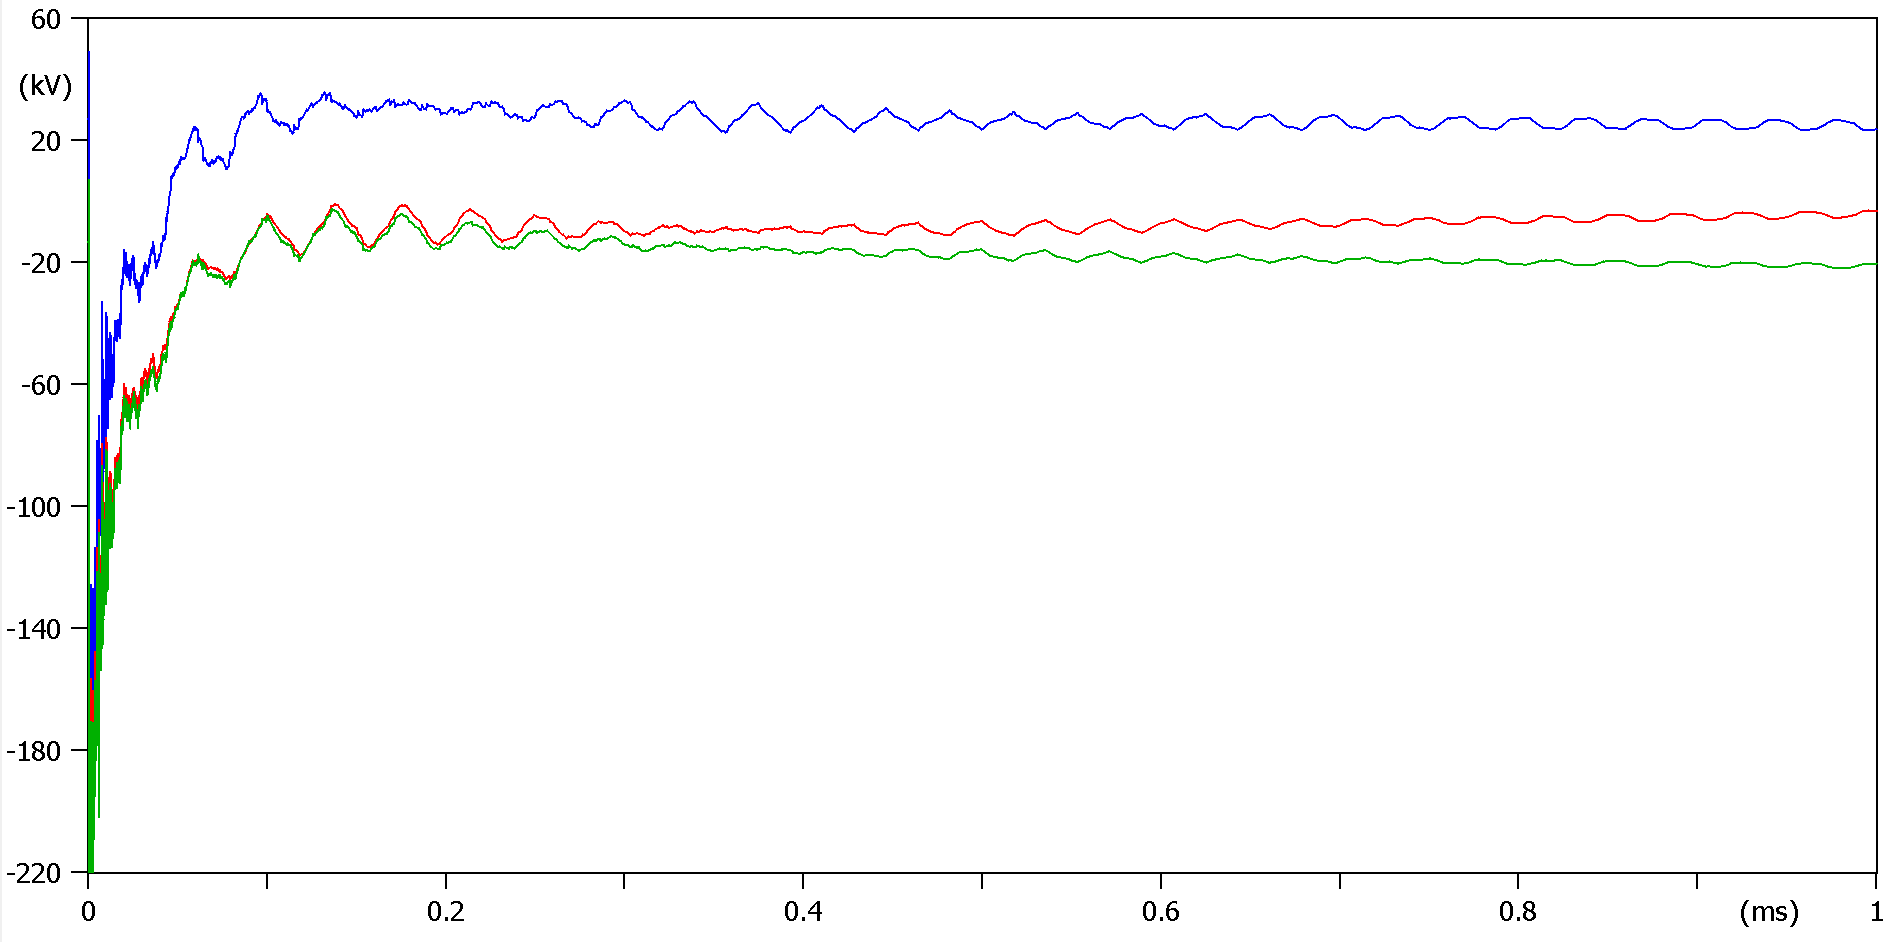
\includegraphics[width=\textwidth]{Figs/Resultados/40m_2.png}
    \caption{Contrapeso de 40 m.}
\end{subfigure}
\hfill
\begin{subfigure}[b]{0.48\textwidth}
    \centering
    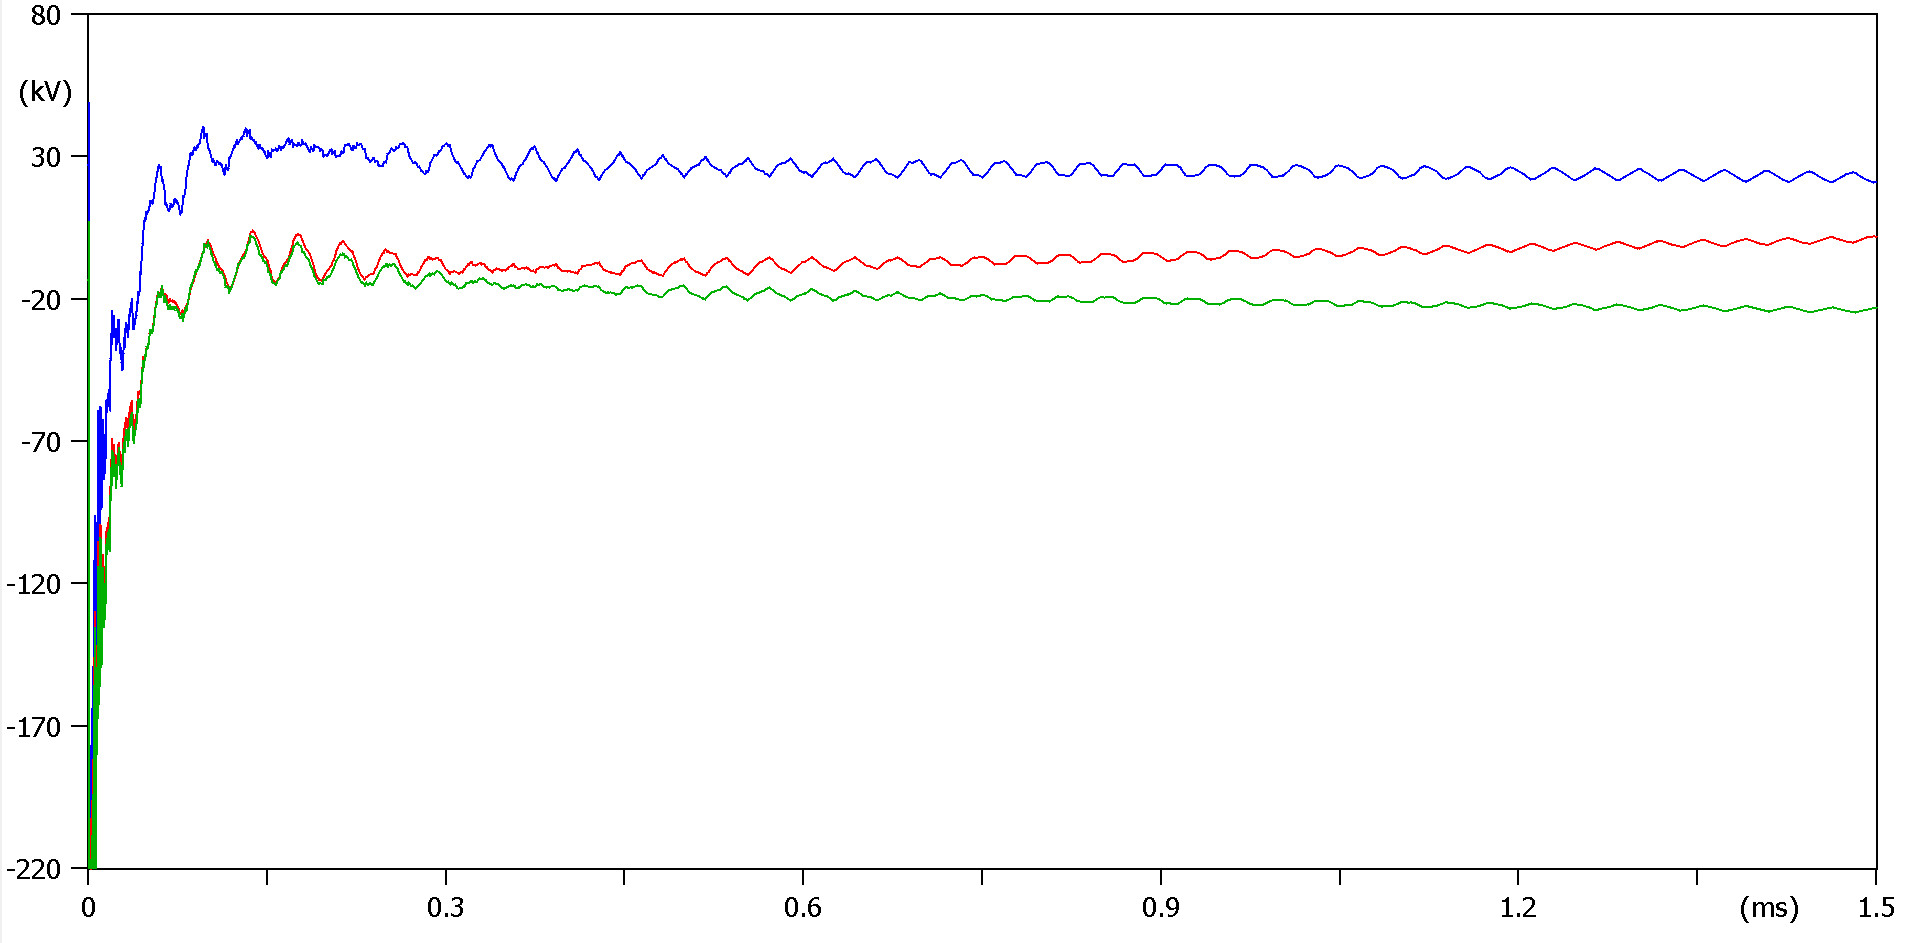
\includegraphics[width=\textwidth]{Figs/Resultados/30m_2.png}
    \caption{Contrapeso de 30 m.}
\end{subfigure}

\vspace{0.3cm}

\begin{subfigure}[b]{0.48\textwidth}
    \centering
    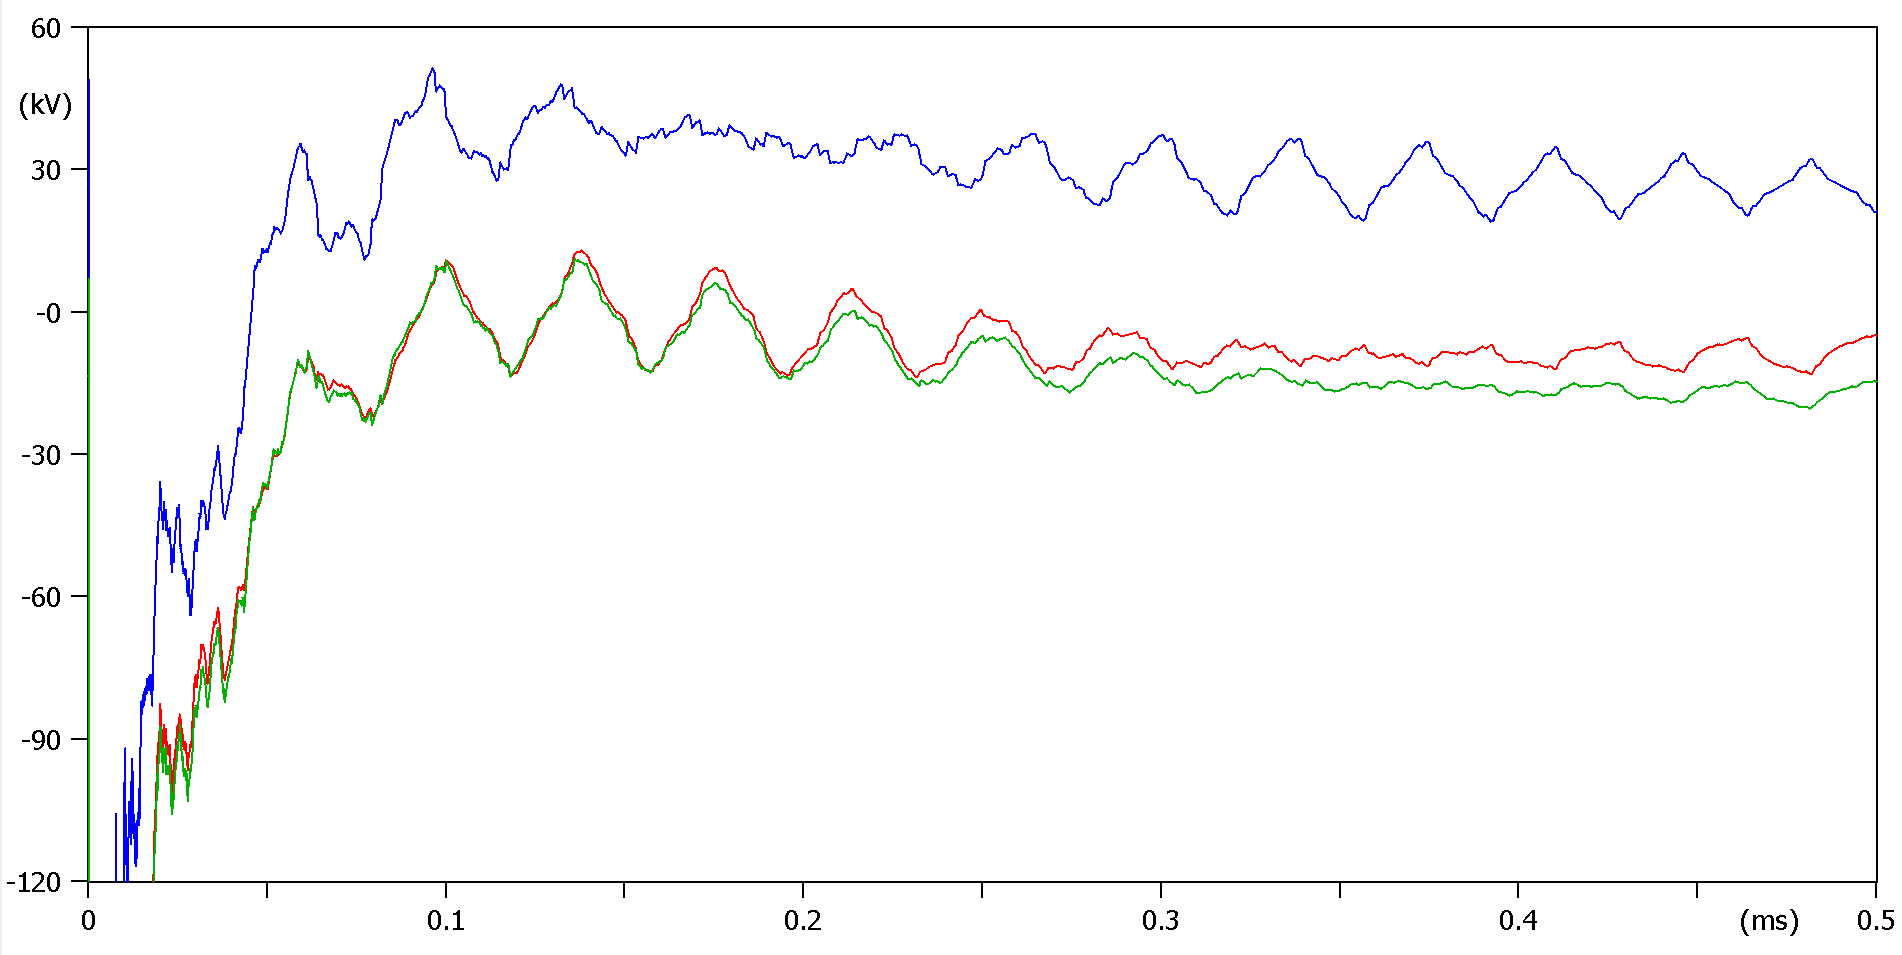
\includegraphics[width=\textwidth]{Figs/Resultados/20m_2.png}
    \caption{Contrapeso de 20 m.}
\end{subfigure}
\hfill
\begin{subfigure}[b]{0.48\textwidth}
    \centering
    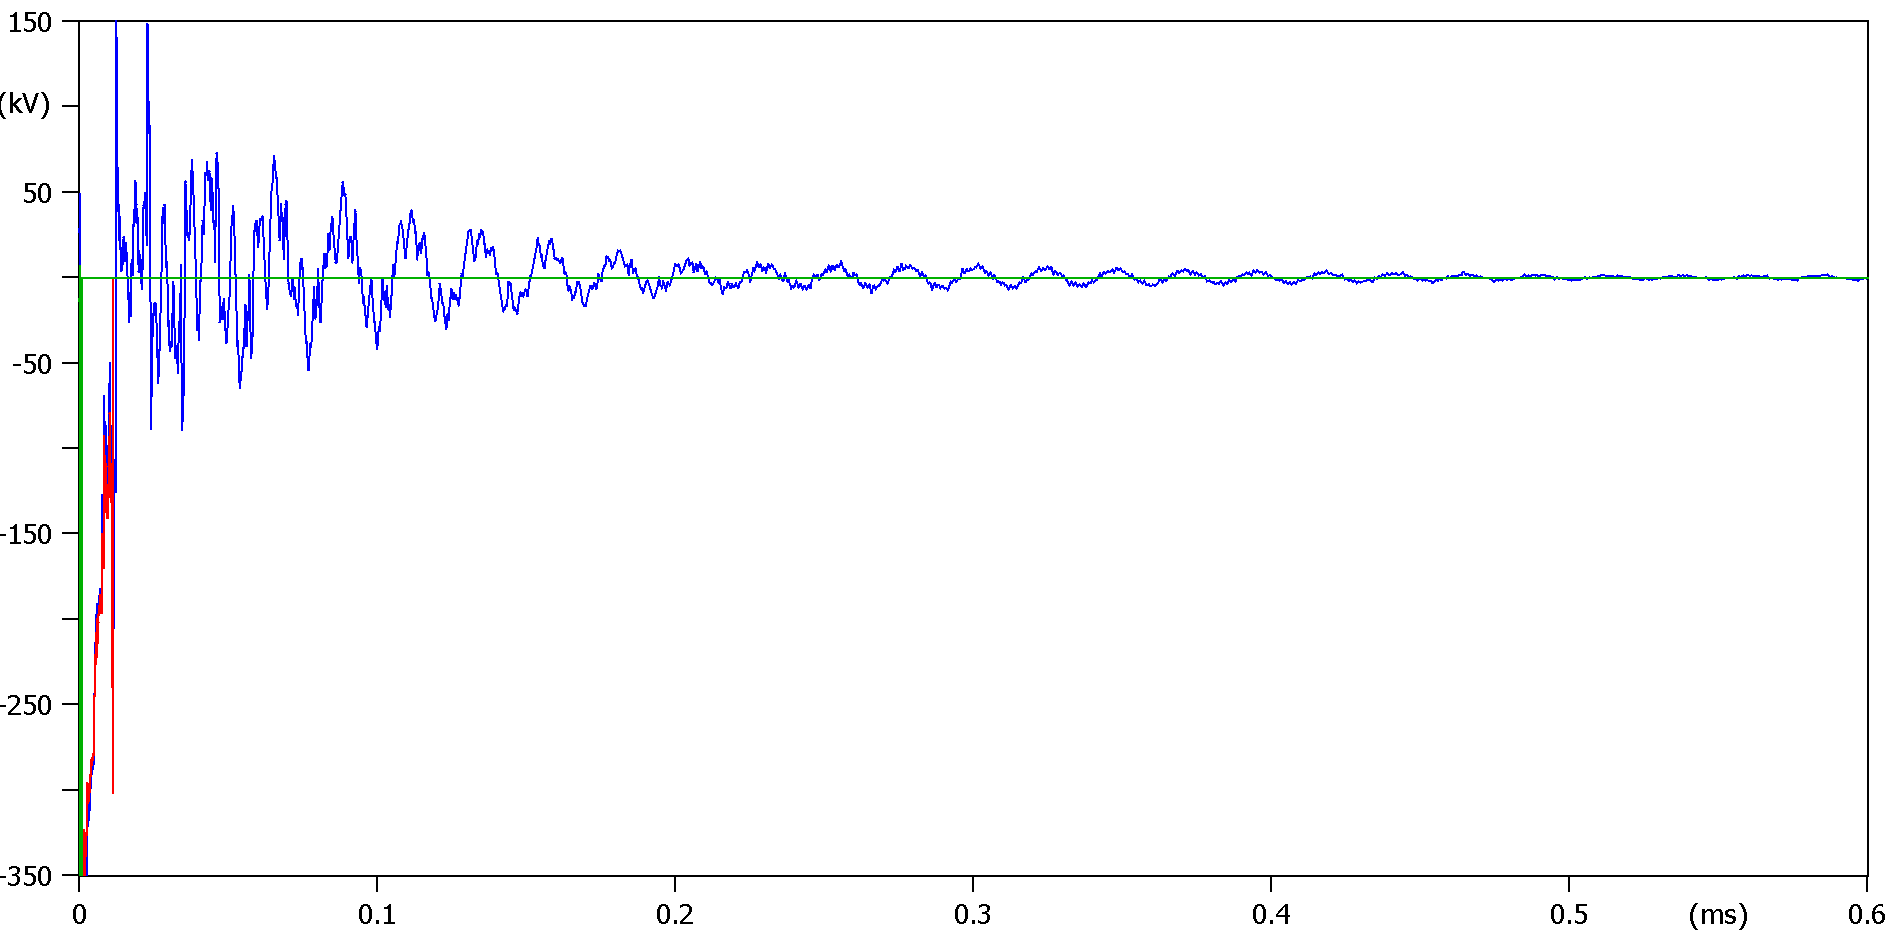
\includegraphics[width=\textwidth]{Figs/Resultados/10m_2.png}
    \caption{Contrapeso de 10 m.}
\end{subfigure}

\caption{Comparación del comportamiento transitorio para las diferentes longitudes de contrapeso evaluadas.}
\label{fig:comparacion_contrapesos}

\end{figure}

Los resultados obtenidos permiten concluir que existe una longitud mínima requerida para garantizar un desempeño adecuado del sistema de puesta a tierra frente a descargas atmosféricas. Aunque las configuraciones de 40 m y 30 m presentaron resultados satisfactorios, la alternativa de 20 m logró mantener la ausencia de \textit{Backflashover} con una menor longitud de conductor enterrado, reduciendo así los requerimientos de instalación y el costo asociado a la implementación.

La configuración de 10 m fue descartada debido a la aparición de fenómenos de ruptura del aislamiento durante las simulaciones transitorias. Por lo tanto, se identificó que la longitud mínima técnicamente aceptable corresponde a 20 m, valor que fue posteriormente utilizado como base para la configuración final del sistema de puesta a tierra.

\section{Conclusiones}

\begin{itemize}
    \item El presente trabajo permitió desarrollar un modelo electromagnético de alta frecuencia de una línea de subtransmisión de 33 kV mediante ATPDraw, incorporando la representación detallada de los apoyos, las cadenas de aislamiento, la descarga atmosférica mediante la función de Heidler y el sistema de puesta a tierra. La implementación de estos elementos permitió reproducir adecuadamente los fenómenos transitorios asociados al impacto de rayos y evaluar el comportamiento de la estructura frente a eventos de \textit{Backflashover}.

    \item Las simulaciones realizadas evidenciaron que la longitud de los contrapesos horizontales constituye una de las variables con mayor influencia sobre el desempeño atmosférico del sistema de puesta a tierra. La reducción progresiva de la longitud de los contrapesos permitió identificar que una configuración de 20 m representa la longitud mínima capaz de evitar la ocurrencia de fenómenos de \textit{Backflashover}, mientras que una longitud de 10 m resultó insuficiente para disipar adecuadamente la corriente impulsiva generada por la descarga atmosférica.

    \item La configuración final seleccionada, compuesta por dos contrapesos horizontales de 20 m y un electrodo vertical de 2.4 m, permitió obtener una resistencia equivalente a pie de torre de $11.6454\ \Omega$. Esta solución logró reducir la elevación de potencial de la estructura durante los eventos transitorios y proporcionar una trayectoria efectiva para la disipación de corriente hacia el terreno, mejorando significativamente el desempeño del sistema respecto a la configuración inicial.

    \item La evaluación estadística realizada mediante IEEE Flash confirmó que el mecanismo predominante de falla en el nodo analizado corresponde al fenómeno de \textit{Backflashover}, el cual representa la mayor contribución a la tasa total de salidas de la línea. Asimismo, los resultados evidenciaron que el sistema de apantallamiento presenta un desempeño satisfactorio, registrándose una baja incidencia de fallas por apantallamiento en comparación con las fallas asociadas a la elevación del potencial de la estructura.

    \item Adicionalmente, sería de interés contrastar los resultados obtenidos mediante simulación con mediciones de campo o información histórica de fallas, con el fin de validar el modelo desarrollado bajo condiciones reales de operación.

    \item Finalmente, el desarrollo de este trabajo representó una valiosa experiencia de aprendizaje en el análisis del desempeño atmosférico de líneas de subtransmisión y en la aplicación de herramientas especializadas de simulación. La integración de conceptos relacionados con descargas atmosféricas, coordinación de aislamiento, modelado electromagnético y sistemas de puesta a tierra permitió fortalecer tanto los conocimientos teóricos como las habilidades prácticas necesarias para abordar problemas reales de ingeniería eléctrica.

\end{itemize}


\section{Bibliografía}
\bibliography{references}

\appendix

\section{Parámetros LCC}
En este anexo se presentan ejemplos de las configuraciones empleadas en el módulo \textit{Line Constants Program} (LCC) para la obtención de los parámetros distribuidos de la línea. Los apoyos A170 y A171 se muestran como referencia del procedimiento utilizado para parametrizar cada vano a partir de la información geométrica suministrada, incluyendo posiciones horizontales de los conductores, alturas de instalación, flechas y resistividad del terreno.

La transición entre ambos apoyos permite evidenciar la actualización de los parámetros geométricos realizada para cada tramo antes de ejecutar el cálculo de las constantes eléctricas de línea.


\begin{figure}[H]
\centering

\begin{subfigure}[b]{0.48\textwidth}
\centering
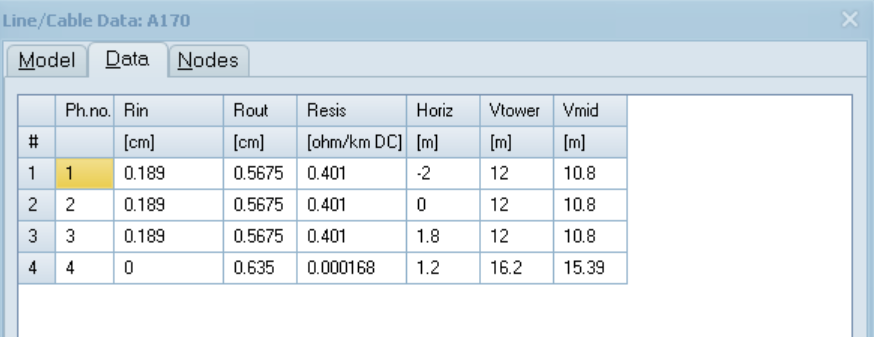
\includegraphics[width=\textwidth]{Figs/Anexos/LCC_A170.png}
\caption{Configuración del apoyo A170.}
\end{subfigure}
\hfill
\begin{subfigure}[b]{0.48\textwidth}
\centering
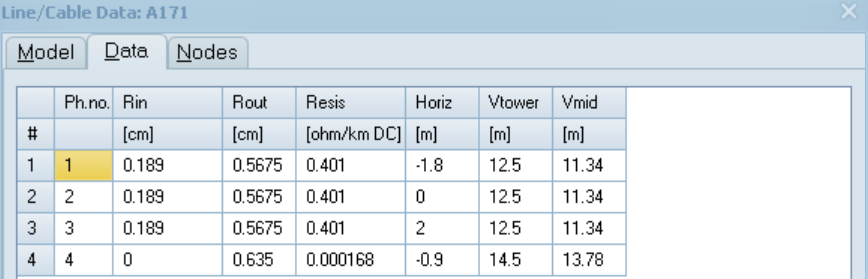
\includegraphics[width=\textwidth]{Figs/Anexos/LCC_A171.png}
\caption{Configuración del apoyo A171.}
\end{subfigure}

\caption{Ejemplo de parametrización geométrica empleada en LCC para la obtención de las constantes de línea.}
\label{fig:lcc_parametrizacion}
\end{figure}

\section{Memorias de cálculo}

Las memorias de cálculo desarrolladas en \textit{SMath Studio} se incluyen como documento complementario al presente informe. En dichas memorias se encuentran detallados los procedimientos de cálculo empleados para la determinación de:

\begin{itemize}
    \item Impedancias de impulso de los apoyos.
    \item Tiempos de propagación de postes, crucetas y bayonetas.
    \item Parámetros distribuidos de los contrapesos horizontales.
    \item Parámetros distribuidos de los electrodos verticales.
    \item Evaluación de las diferentes configuraciones analizadas durante el proceso de optimización.
\end{itemize}

Debido a la extensión de los desarrollos matemáticos, estos se presentan de forma íntegra en el archivo adjunto \textit{Memoria de Cálculo SMath G4.pdf}, el cual constituye el soporte técnico de los resultados mostrados en este documento.

\section{Modelos ATPDraw}
En este anexo se presentan los modelos electromagnéticos implementados en ATPDraw para la evaluación del desempeño frente a descargas atmosféricas del tramo asignado.

\begin{figure}[H]
\centering
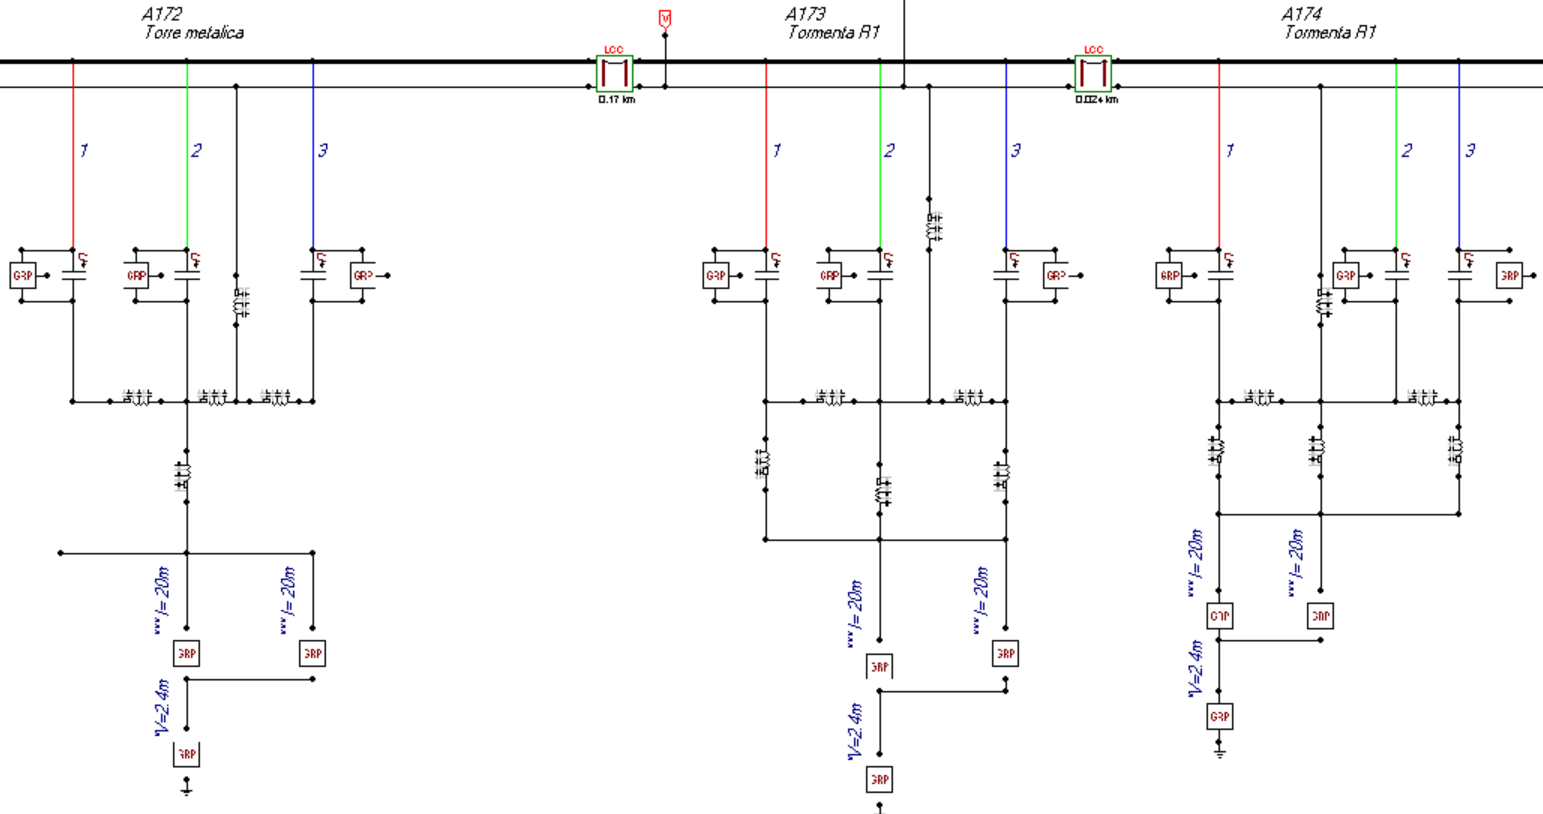
\includegraphics[width=0.75\textwidth]{Figs/Anexos/Modelo_estudio.png}
\caption{Modelo electromagnético implementado para los apoyos de estudio A172, A173 y A174, incluyendo aisladores, impedancias de impulso y sistema de puesta a tierra optimizado.}
\label{fig:modelo_detallado}
\end{figure}

\begin{figure}[H]
\centering
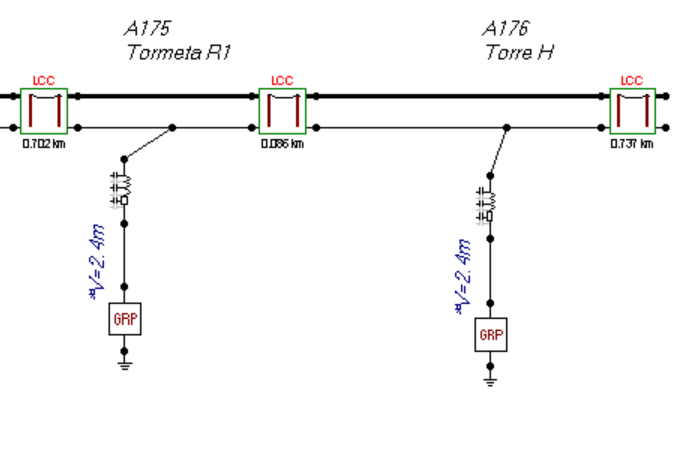
\includegraphics[width=0.65\textwidth]{Figs/Anexos/Modelo_sim.png}
\caption{Representación simplificada de los apoyos adyacentes mediante impedancias equivalentes y modelos de puesta a tierra distribuidos.}
\label{fig:modelo_simplificado}
\end{figure}


\section{Resultados IEEE Flash}


La Figura~\ref{fig:ieee_flash_final} presenta la configuración final evaluada en IEEE Flash para el apoyo A173, correspondiente al diseño seleccionado de puesta a tierra compuesto por dos contrapesos horizontales de 20~m y un electrodo vertical de 2.4~m.
\begin{figure}[H]
\centering
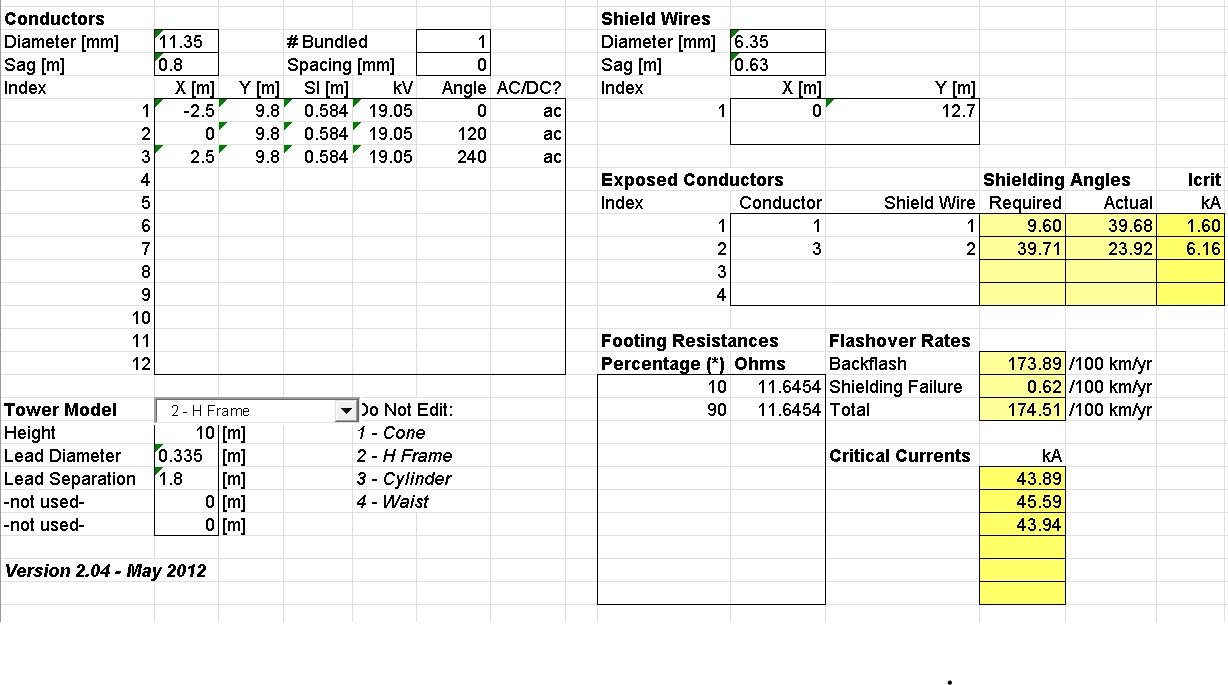
\includegraphics[width=\textwidth]{Figs/Anexos/Flash_general.jpg}
\caption{Resultados obtenidos en IEEE Flash para la configuración final seleccionada del apoyo A173.}
\label{fig:ieee_flash_final}
\end{figure}

\section{Archivos Complementarios Entregados}

Junto con el presente informe se suministran los siguientes archivos digitales:

\begin{itemize}
	\item Archivo de simulación ATPDraw (.acp), correspondiente al modelo electromagnético desarrollado para el nodo de estudio.
	
	\item Archivo de cálculo SMath Studio (.sm), que contiene las memorias de cálculo utilizadas para la determinación de impedancias de impulso, parámetros de puesta a tierra y demás cálculos requeridos durante el desarrollo del proyecto.
	
	\item Archivo Microsoft Excel (.xlsx) asociado a IEEE Flash 2.04, utilizado para la evaluación estadística del desempeño de la estructura frente a descargas atmosféricas, correspondiente al entregable establecido en el Taller 2.
\end{itemize}

Estos archivos complementan la información presentada en el informe y permiten reproducir los cálculos, simulaciones y análisis efectuados durante el desarrollo del trabajo.


\end{document}
